\documentclass[a4paper]{article}

%% Language and font encodings
\usepackage[english]{babel}
\usepackage[utf8x]{inputenc}
\usepackage[T1]{fontenc}

%% Sets page size and margins
\usepackage[a4paper,top=3cm,bottom=2cm,left=3cm,right=3cm,marginparwidth=1.75cm]{geometry}

%% Useful packages
\usepackage{amsmath}
\usepackage{graphicx}
\usepackage[colorinlistoftodos]{todonotes}
\usepackage[colorlinks=true, allcolors=blue]{hyperref}
\usepackage{float}
\usepackage{enumerate}
\usepackage{subfig}
\setlength\parindent{0pt}
\usepackage{amssymb}
\setcounter{section}{-1}
\title{MA 503 : Lebesgue Measure and Integration}
\author{Dane Johnson}

\begin{document}
\maketitle

\section*{Chapter 2 : The Real Number System}

\subsection*{1 Axioms for the Real Numbers}

{\bf C. Completeness Axiom} Every nonempty set $S$ of real numbers which has an upper bound has a least upper bound.\\


{\bf 1. Proposition} Let $L$ and $U$ be nonempty subsets of $\mathbb{R}$ such that $\mathbb{R} = L \cup U$ and such that for each $l \in L$ and for each $u \in U$, $l<u$. Then either $L$ has a greatest element of $U$ has a least element.\\

{\bf Problem 3}

Prove Proposition 1 using Axiom C.\\

Proof: The statement that either $L$ has a greatest element or $U$ has a least element is equivalent to the statement that if $U$ does not have a least element then $L$ must have a greatest element. Suppose $U$ does not have a least element and let $u \in U$ be arbitrary. Since $l<u$ for all $l \in L$, $u$ is an upper bound of $L$ so $L$ has a least upper bound, which we denote sup $L$. Since $u$ was arbitary and sup $L$ is the least upper bound of $L$, we have sup $L \leq u$ for all $u \in U$. Therefore, sup $L \leq $ inf $U$. Suppose that sup $L$ is not an element of $L$. Then since $\mathbb{R} = L \cup U$, it follows that sup $L$ is an element of $U$. Since inf $U \leq u$ for every element $u \in U$, this means inf $U \leq $ sup $L$. Thus inf $U = $ sup $L$. This means that sup $L$ is an element of $U$, less than or equal to any element of $U$. That is, sup $L$ is the least element of $U$. This contradicts the assumption that $U$ does not have a least element. So it must be the case that sup $L$ is an element of $L$. Since sup $L$ is greater than or equal to any element of $L$, sup $L$ is the greatest element of $L$. \\

\subsection*{2 The Natural and Rational Numbers as Subsets of $\mathbb{R}$}

{\bf Axiom of Archimedes} For any real number $x$, there is an integer $n$ such that $x<n$.\\

{\bf Corollary 4} Between any two real numbers is a rational; that is, if $x<y$ there is a rational $r$ with $x<r<y$. \\

\subsection*{4 Sequences of Real Numbers}

{\bf Definition} For a sequence $(x_n)$, we say that lim $x_n = \infty$ if given $\Delta$, there is an $N$ such that for all $n\geq N$, $x_n > \Delta$. Equivalently, if given $\Delta$, there is an $N$ such that for all $n\geq N$, $x_n \geq \Delta$. The case for lim $x_n = -\infty$ is defined similarly. The definition of lim $x_n = l \in \mathbb{R}$ is standard and omitted from these notes. \\

{\bf Problem 7}\\
Show that a sequence can have at most one limit.\\

Suppose that $l$ and $l'$ are both limits of the sequence $(x_n)$. Let $\epsilon > 0$ be arbitrary. There exist natural numbers $N_1$ and $N_2$ such that $|x_n -l| < \epsilon / 2$ for all $n > N_1$ and $|x_n - l'| < \epsilon / 2$ for all $n > N_2$. Take $N = $ max$\{N_1,N_2\}$. Then for all $n > N$, $|x_n - l| + |x_n - l'| < \epsilon$. But since $|l - l'| = |l - x_n + x_n - l'| \leq |x_n - l| + |x_n - l'|$, this shows that $|l-l'| < \epsilon$. Since this holds for any $\epsilon >0$, we have $|l - l'| \leq 0$. Because  $0\leq |l-l'|$ as well, conclude that $l =l'$. \\

{\bf Definition} We say that $l$ is a {\bf cluster point} of $(x_n)$ if, given $\epsilon > 0$ and given $N \in \mathbb{N}$, there exists an $n \geq N$ such that $|x_n - l| < \epsilon$. To extend this to the case that $l = \infty$, we say that $l = \infty$ is a cluster point of $(x_n)$ if, given $\Delta$ and given $N$, there exists an $n \geq N$ such that $x_n \geq \Delta$. The case for $l= -\infty$ is defined similarly. \\

{\bf Problem 8}\\
Show that $l$ is a cluster point of the sequence $(x_n)$ if and only if $(x_n)$ has a subsequence $(x_{n_j})$ that converges to $l$.\\

The textbook allows $l = \infty$ or $l = -\infty$. First consider the case that $l$ is finite. \\

Let $l$ be a cluster point of $(x_n)$. There exists an $n_1 \geq 1$ such that $|x_{n_1} - l| < 1$. Next, since $n_1 \in \mathbb{N}$ and 1/2 > 0, there exists an $n_2 \geq n_1$ such that $|x_{n_2} - l| < 1/2$. Continue in this way to construct a subsequence $(x_{n_j})$ of $(x_n)$ such that for each $j \geq 2$, we can find a natural number $n_j$ such that $n_j \geq n_{j-1}$ and for which $|x_{n_j} - l| < 1/j$. Since $1/j \rightarrow 0$ as $j \rightarrow \infty$, the subsequence $(x_{n_j})$ converges to $l$. \\

Suppose that $(x_{n_j})$ is a subsequence of $(x_n)$ such that $(x_{n_j})$ converges to $l$. Let $\epsilon >0$ and $N \in \mathbb{N}$. Since $(x_{n_j})$ converges to $l$, there exists a $J \in \mathbb{N}$ such that for all $j \geq J$, $|x_{n_j} -l| \leq \epsilon$. If $N \leq n_J$, then $n_J$ is a natural number greater than or equal to $N$ such that $|x_{n_J} - l| < \epsilon$ and we are finished (note that any term in the subsequence, such as $x_{n_J}$, is also a term in the sequence original sequence $(x_n)$). Otherwise if $N > n_j$, then $N \geq N$ and $|x_{N} - l|< \epsilon$. This shows that for any $\epsilon > 0 $ and for any $N \in \mathbb{N}$, there exists an $n\in \mathbb{N}$ such that $n \geq N$ and $|x_n - l| < \epsilon$. \\

Let $l = \infty$ be a cluster point of $(x_n)$. There exists an $n_1 \geq 1$ such that $x_{n_1} \geq 1$. Next there exists an $n_2 \geq n_1$ such that $x_{n_2} \geq 2$. Continue in this way to construct a subsequence $(x_{n_j})$ of $(x_n)$ such that for each $j \geq 2$, we can find an $n_j \geq n_{j-1}$ such that $x_{n_j} \geq j$. But this shows that $x_{n_j} \rightarrow \infty = l$ as $j \rightarrow \infty$. For $l = -\infty$ we use very similar reasoning except that we construct a subsequence $(x_{n_j})$ such that $x_{n_j} < -j$ for each $j \in \mathbb{N}$ so that $x_{n_j} \rightarrow -\infty = l$ as $j \rightarrow \infty$. \\

{\bf Definition} For a nonempty set of real numbers $S$, we write sup $S = \infty$ if $S$ is not bounded above. This means that given $\Delta$, there exists an element $s \in S$ such that $s > \Delta$ (or equivalently such that $s \geq \Delta$). We write inf $S = -\infty$ if $S$ is not bounded below. This means that given $\Delta$, there exists an element $s \in S$ such that $s < \Delta$ (or equivalently such that $s \leq \Delta$).\\

{\bf Definition} We define the limit superior and limit inferior of the sequence $(x_n)$ as

$$\text{lim sup } x_n = \text{inf}_{k\in \mathbb{N}} (\text{sup}_{n \geq k} \, x_n)$$
$$\text{lim inf } x_n =\text{sup}_{k \in \mathbb{N}} (\text{inf}_{n\geq k} \, x_n) \;.$$

{\bf Remark} For a real valued sequence $(x_n)$, the limit superior and limit inferior always exist in $\overline{\mathbb{R}}$ and 
$$\text{sup}_{k \in \mathbb{N}} (\text{inf}_{n\geq k} \, x_n) = \text{lim}_{k\rightarrow \infty} (\text{inf}_{n\geq k} \, x_n) \in [-\infty, \infty]$$
$$\text{inf}_{k \in \mathbb{N}} (\text{sup}_{n\geq k} \, x_n) = \text{lim}_{k\rightarrow \infty} (\text{sup}_{n\geq k} \, x_n) \in [-\infty, \infty] \;.$$

Proof:\\

Consider that the sequence (inf$_{n\geq k}\, x_n)_{k=1}^{\infty}$ $\subset [-\infty, \infty)$ is an increasing sequence and must converge to its supremum in $\overline{\mathbb{R}}$. The sequence (sup$_{n\geq k}\, x_n)_{k=1}^{\infty}$ $\subset (-\infty, \infty]$ is a decreasing sequence and must converge to is infimum in $\overline{\mathbb{R}}$. This means the limit superior and limit inferior always exist and may indeed be written as the improper limits stated above.\\

{\bf Remark} The extended real number $\infty$ is the limit superior of $(x_n)$ if and only if given $\Delta$ and $k$, there is an $n\geq k$ such that $x_n > \Delta$. The extended real number $-\infty$ is the limit inferior of $(x_n)$ if and only if given $\Delta$ and $k$, there is an $n\geq k$ such that $x_n < \Delta$.\\

Proof:
\begin{align*}
&\infty = \text{inf}_{k \in \mathbb{N}}(\text{sup}_{n\geq k} x_n) \\
&\iff \infty \leq \text{inf}_{k \in \mathbb{N}}(\text{sup}_{n\geq k} x_n)\\
&\iff \infty \leq \text{sup}_{n\geq k} x_n   \quad \forall k \in \mathbb{N}\\
&\iff \infty=\text{sup}_{n\geq k} x_n  \quad (\forall k \in \mathbb{N)}\\
&\iff \{x_n \;|\; n\geq k\} \text{ is not bounded above} \quad (\forall k \in \mathbb{N})\\
&\iff \text{Given } \Delta, \text{there is an element } x_n \in \{x_n \;|\; n\geq k\} \text{ s.t. } x_n> \Delta \quad (\forall k \in \mathbb{N})\\
&\iff \text{Given }\Delta \text{ and } k, \text{ there is an } x_n \text{ s.t. } n\geq k \text{ and } x_n > \Delta.
\end{align*}

\begin{align*}
&-\infty = \text{sup}_{k \in \mathbb{N}}(\text{inf}_{n\geq k} x_n) \\
&\iff -\infty \geq \text{sup}_{k \in \mathbb{N}}(\text{inf}_{n\geq k} x_n)\\
&\iff -\infty \geq \text{inf}_{n\geq k} x_n   \quad \forall k \in \mathbb{N}\\
&\iff -\infty=\text{inf}_{n\geq k} x_n  \quad (\forall k \in \mathbb{N)}\\
&\iff \{x_n \;|\; n\geq k\} \text{ is not bounded below} \quad (\forall k \in \mathbb{N})\\
&\iff \text{Given } \Delta, \text{there is an element } x_n \in \{x_n \;|\; n\geq k\} \text{ s.t. } x_n< \Delta \quad (\forall k \in \mathbb{N})\\
&\iff \text{Given }\Delta \text{ and } k, \text{ there is an } x_n \text{ s.t. } n\geq k \text{ and } x_n < \Delta.
\end{align*}

{\bf Remark} The extended real number $-\infty$ is the limit superior of $(x_n)$ if and only if lim $x_n = -\infty$. The extended real number $\infty$ is the limit inferior of $(x_n)$ if and only if lim $x_n = \infty$.\\

Proof:\\

\begin{align*}
&-\infty = \text{inf}_{k\in \mathbb{N}}\text{sup}_{n\geq k} x_n = \text{inf}\{\text{sup} \{x_n : n \geq k\} : k \in \mathbb{N}\}\\
&\iff \text{inf}\{\text{sup} \{x_n : n \geq k\} : k \in \mathbb{N}\} \text{ is not bounded below}\\
&\iff \text{Given } \Delta, \exists k \text{ s.t. } \text{sup}\{x_n : n \geq k\} \leq \Delta\\
&\iff \text{Given } \Delta, \exists k \text{ s.t. } \forall n\geq k, x_n \leq \Delta \\
&\iff \text{lim } x_n = -\infty\;.
\end{align*}

\begin{align*}
&\infty = \text{sup}_{k\in \mathbb{N}}\text{inf}_{n\geq k} x_n = \text{sup}\{\text{inf} \{x_n : n \geq k\} : k \in \mathbb{N}\}\\
&\iff \text{sup}\{\text{inf} \{x_n : n \geq k\} : k \in \mathbb{N}\} \text{ is not bounded above}\\
&\iff \text{Given } \Delta, \exists k \text{ s.t. } \text{inf}\{x_n : n \geq k\} \geq \Delta\\
&\iff \text{Given } \Delta, \exists k \text{ s.t. } \forall n\geq k, x_n \geq \Delta \\
&\iff \text{lim } x_n = \infty\;.
\end{align*}

{\bf Remark} A real number $l$ is the limit superior of the sequence $(x_n)$ if and only if both\\
(i) given $\epsilon >0$, $\exists k$ such that $x_n < l+\epsilon$ for all $n \geq k$ and \\
(ii) given $\epsilon >0$ and given $k$, $\exists n \geq k$ such that $x_n > l - \epsilon$.\\

Proof:\\

Let $\epsilon > 0$ be arbitrary and let $l = \text{inf}\{\text{sup} \{x_n : n \geq k\} : k \in \mathbb{N}\}$.\\

By definition of infimum, there exists a $k$ such that $\text{sup} \{x_n : n \geq k\} < l+\epsilon$. By definition of supremum, this means there is a $k$ such that $x_n < l + \epsilon$ for all $n \geq k$. So if $l$ is the limit superior of $(x_n)$, then (i) holds. \\

Let $k$ be given. Since $l-\epsilon < l = \text{inf}\{\text{sup} \{x_n : n \geq k\} : k \in \mathbb{N}\}$, we have $l-\epsilon<l\leq \text{sup} \{x_n : n \geq k\}$ for any $k$ and therefore in particular the given $k$. This means that $l-\epsilon$ is not an upper bound of the set $\text{sup} \{x_n : n \geq k\}$ (for the given $k$), so there exists an element $x_n \in \text{sup} \{x_n : n \geq k\}$ such that $l-\epsilon < x_n$. That is, for $k$ given, there is an $n\geq k$ such that $l-\epsilon < x_n$. So if $l$ is the limit superior of $(x_n)$ then (ii) holds as well.\\

We have shown that if $l$ is the limit superior of $(x_n)$, then both conditions (i) and (ii) hold.\\

Next suppose that both conditions (i) and (ii) hold for a real number $l$.\\

For any $\epsilon > 0$, there exists by (i) a $k \in \mathbb{N}$ such that $x_n < l+\epsilon$ for all $n\geq k$. So there exists a $k$ such that $\text{sup} \{x_n : n \geq k\} \leq l+\epsilon$. By definition of infimum, $\text{inf}\{\text{sup} \{x_n : n \geq k\} : k \in \mathbb{N}\} \leq \text{sup} \{x_n : n \geq k\} \leq l+\epsilon$. Since this inequality holds for all $\epsilon > 0$, we have $\text{inf}\{\text{sup} \{x_n : n \geq k\} : k \in \mathbb{N}\} \leq l$. \\

Since (ii) holds we have for any $k \in \mathbb{N}$, that given any $\epsilon >0$ there is an $n\geq k$ such that $l-\epsilon < x_n$. Since $x_n \leq \text{sup} \{x_n : n \geq k\}$, this means that for all $k$, given $\epsilon>0$, it follows that $l-\epsilon < \text{sup} \{x_n : n \geq k\}$. Since this inequality holds for all $\epsilon >0$, $l \leq \text{sup} \{x_n : n \geq k\}$ for all $k$. This shows that $l$ is a lower bound of the set $\{\text{sup} \{x_n : n \geq k\} : k \in \mathbb{N}\}$ and so $\text{inf}\{\text{sup} \{x_n : n \geq k\} : k \in \mathbb{N}\} \leq l$.\\

We have shown that if (i) holds, then lim sup $x_n \leq l$ and if (ii) holds, then lim sup $x_n \geq l$. Therefore, if both (i) and (ii) hold for a real number $l$, then lim sup $x_n = l$ as proposed. \\

{\bf Remark} A real number $l$ is the limit inferior of the sequence $(x_n)$ if and only if both\\
(i) given $\epsilon >0$, $\exists k$ such that $x_n > l-\epsilon$ for all $n \geq k$ and \\
(ii) given $\epsilon >0$ and given $k$, $\exists n \geq k$ such that $x_n < l + \epsilon$.\\

Proof:\\
The proof of this remark is similar to the proof of the previous remark by modifying signs and directions of inequalities.\\

{\bf Remark} lim sup $(-x_n)$ = $-$lim inf $(x_n)$.\\

Proof:\\

For a set $A$ of real numbers, sup$(-A) = -$inf$(A)$. For each $-a \in A :=\{-a \; : \: a \in A\}$, $-a\leq$ sup$(-A)$, so $a \geq -$sup$(-A)$ for all $a \in A$. By definition of infimum, inf$(A) \geq -$sup$(-A)$ and $-\text{inf}(A) \leq $sup$(-A)$.  We have $a \geq $inf$(A)$ for all $a \in A$ and so $-a \leq -$inf$(A)$ for all $-a \in -A$. By definition of supremum, sup$(-A) \leq -$inf$(A)$. Therefore sup$(-A) = -\text{inf}(A)$. Here this means,

$$\text{sup}\{-x_n \; | \; x_n \in (x_n) \text { and } n\geq k\} = -\text{inf}\{x_n \; | \; x_n \in (x_n) \text { and } n\geq k\} \quad \forall k \in \mathbb{N} \;.$$
Which means in more compact notation,
$$\text{sup}_{n\geq k} (-x_n) = -\text{inf}_{n\geq k} x_n \quad \forall k \in \mathbb{N} \;.$$
$$\therefore \text{lim sup } (-x_n) = \text{lim}_{k\rightarrow \infty} \text{sup}_{n\geq k} (-x_n) = \text{lim}_{k\rightarrow \infty}(- \text{inf}_{n\geq k} x_n) = -\text{lim}_{k\rightarrow \infty}\text{inf}_{n\geq k} x_n = -\text{lim inf} x_n \;.$$

\textbf{Remark} lim inf $x_n \leq $ lim sup $x_n$.\\

Proof:\\

For each $k$, inf$_{n\geq k} x_n \leq x_n$ for all $n\geq k$ and $x_n \leq $sup$_{n\geq k}$ for all $n\geq k$. Thus, for each $k$, inf$_{n\geq k} x_n \leq$sup$_{n\geq k}$. Therefore by either taking $k\rightarrow \infty$ or alternatively by using this inequality and the definitions of supremum and infimum in turn the claim follows. \\


{\bf Remark} If $(x_n)$ and $(y_n)$ are two sequences,

\begin{align*}
\text{lim inf } x_n + \text{ lim inf } y_n &\leq \text{ lim inf }(x_n+y_n)\\
&\leq \text{lim sup } x_n + \text{ lim inf } y_n\\
&\leq \text{ lim sup } (x_n + y_n)\\
&\leq \text{ lim sup }x_n + \text{ lim sup } y_n
\end{align*}

Proof:\\

For sets $A$ and $B$, inf $A \leq a$ for all $a \in A$ and inf $B \leq b$ for all $b \in B$. So inf $A + $ inf $B \leq a+b$ for all $a \in A$, $b \in B$. Therefore inf $A + $ inf $B \leq $ inf $(A+B)$. Here,
$$\text{inf}_{n\geq k} x_n + \text{inf}_{n\geq k} y_n \leq \text{inf}_{n\geq k} (x_n + y_n) \quad \forall k \in \mathbb{N} \;.$$

Passing to the limit $k\rightarrow \infty$ establishes the first inequality. \\

For any fixed $k$,

$$\text{inf}_{n\geq k} (x_n + y_n) \leq x_l + y_l \leq \text{sup}_{n\geq k} x_n + y_l \quad \forall l\geq k$$
$$\implies \text{inf}_{n\geq k} (x_n + y_n) - \text{sup}_{n\geq k} x_n\leq y_l \quad \forall l \geq k$$
$$\implies \text{inf}_{n\geq k} (x_n + y_n) - \text{sup}_{n\geq k} x_n\leq \text{inf}_{n\geq k} y_n$$
$$\implies \text{inf}_{n\geq k} (x_n + y_n) \leq \text{sup}_{n\geq k} x_n + \text{inf}_{n\geq k} y_n \;.$$

Passing to the limit $k\rightarrow \infty$ establishes the second inequality. Bidirectional arrows could have been used but would not help in what we want to prove.\\

The next inequality is proved similar to the previous one so will the steps will be abbreviated. For any $k$,

$$x_l + \text{inf}_{n\geq k} y_n \leq \text{sup}_{n\geq k} (x_n + y_n) \quad \forall l \geq k$$
$$\implies \text{sup}_{n\geq k} x_n  + \text{inf}_{n\geq k} y_n \leq \text{sup}_{n\geq k} (x_n + y_n) \;.$$

Passing to the limit $k\rightarrow \infty$ establishes the third inequality. \\

Since $x_l \leq \text{sup}_{n\geq k} x_n $ for all $l\geq k$ and $y_l \leq \text{sup}_{n\geq k} y_n$ for all $l \geq k$, $x_l + y_l \leq \text{sup}_{n\geq k} x_n + \text{sup}_{n\geq k} y_n$ for all $l\geq k$. Thus by definition of supremum, $\text{sup}_{n\geq k} (x_n+y_n) \leq \text{sup}_{n\geq k} x_n + \text{sup}_{n\geq k} y_n$. Passing to the limit $k\rightarrow \infty$ establishes the fourth inequality. \\

{\bf Problem 9}\\
{\bf a.} Show that lim sup $x_n$ and lim inf $x_n$ are respectively the largest and smallest cluster points of the sequence $(x_n)$. \\


Write $u = $inf$_{k\in \mathbb{N}} $ sup$_{n \geq k} \; x_n$ to denote the limit supremum of the sequence $(x_n)$. First we will establish that $u$ is a cluster point of $(x_n)$ and then afterward show that if $c$ is a cluster point of $(x_n)$, $c\leq u$. We have separate definitions for limit supremum depending on whether the limit supremum is finite, $\infty$, or $-\infty$ and similarly for a cluster point. \\


If $u \in \mathbb{R}$, then to show that $u \in \mathbb{R}$ is a cluster point of $(x_n)$, we need to show that given $\epsilon$ and given $N \in \mathbb{N}$ there is an $n \geq N$ such that $|x_n-u| < \epsilon$. Since $u$ is the limit superior of $(x_n)$, it follows that (i)  there exists a $k_1$ such that for all $n \geq k_1$, $x_n < u + \epsilon$ and (ii) there is a $k_2 \geq N$ such that $u - \epsilon < x_{k_2}$. Take $n^* = $ max$\{N,k_1,k_2\}$ (this is a nonempty finite set, so it is bounded, has a supremum, and contains its supremum). Since $n^* \geq k_1$, $x_{n^*} < u + \epsilon$. Since $n^* \geq k_2$, $u - \epsilon < x_{n^*}$. Therefore, given $\epsilon$ and given $N$, there exists an $n^* \geq N$ such that $u - \epsilon < x_{n^*} < u + \epsilon$, meaning $u$ is a cluster point of $(x_n)$.\\

If $u = \infty$, then given $\Delta$ and $k$, there is an $n \geq k$ such that $x_n > \Delta$. We say that $\infty$ is a cluster point of $(x_n)$ if, given $\Delta$ and given $N$, there exists an $n \geq N$ such that $x_n \geq \Delta$. These definition are equivalent, which can be seen by very minor adjustments. Therefore, $\infty$ is the limit superior of $(x_n)$ if and only if $\infty$ is a cluster point of $(x_n)$. \\

If $u = -\infty$ then lim $x_n = -\infty$, which by definition means that given $\Delta$, there exists a $k$ such that for all $n \geq k$, $x_n < \Delta$. We say that $-\infty$ is a cluster point of $(x_n)$ if given $\Delta$ and given $N$, there is an $n \geq N$ such that $x_n < \Delta$ (the definition is equivalent whether we use $<$ or $\leq$ in this case). So let $\Delta$ and $N$ be given. There exists a $k$ such $n \geq k$, $x_n < \Delta$. If $k \geq N$, then since $k\geq k$, $x_k < \Delta$ as desired. If $N>k$, then $N\geq N$ and $x_N < \Delta$ as desired. Therefore, if $u = -\infty$ is the limit superior of $(x_n)$, $u = -\infty$ is a cluster point of $(x_n)$. \\

\underline{Milestone:} we have shown that if $u$ is the limit superior of $(x_n)$, $u$ is a cluster point of $(x_n)$. Next we need to prove that if $c \in \overline{\mathbb{R}}$ is a cluster point of $(x_n)$ (since the limit superior always exists, we must also always have at least one cluster point), $c\leq u$. The approach is similar to the above in that we consider cases. We have an arbitrary sequence $(x_n)$. This sequence has a limit superior $u$. Either $u \in \mathbb{R}$, $u = \infty$, or $u = -\infty$.\\

Suppose $u \in \mathbb{R}$ and let $c \in \overline{\mathbb{R}}$ be a cluster point of $(x_n)$. Suppose for contradiction that $c>u$. $c-u>0$. There is a $k$ such that for all $n\geq k$, $x_n < u + (c-u)/2$. But this means for all $n\geq k$, $|x_n - c| \geq c - x_n > (c-u)/2$. So for $\epsilon := (c-u)/2 >0$ we have found a natural number $k$ such that there does not exist an $n\geq k$ for which $|x_n-c| < \epsilon$. Thus $c$ cannot be a cluster point of $(x_n)$. This is a contradiction that arose from the assumption $c>u$. Conclude that $c \leq u$ for any cluster point $c$. \\

Suppose $u =\infty$ and let $c \in \overline{\mathbb{R}}$ be a cluster point of $(x_n)$. Assume $c>u$. Then $c>\infty$ which contradicts the fact that $y\leq \infty$ for all $y \in \overline{\mathbb{R}}$. Conclude that $c\leq u$ for any cluster point $c$. \\

Suppose $u =-\infty$ and let $c \in \overline{\mathbb{R}}$ be a cluster point of $(x_n)$. Since $u = -\infty$, lim $x_n = -\infty$. Then lim $x_{n_j} = -\infty$ for any subsequence $(x_{n_j})$ of $(x_n)$ (if not then $(x_{n_j})$ is bounded below and so there must exist some $\Delta$ for which we can not produce a $k$ such that $x_n < \Delta$ for all $n\geq k$ for the original sequence). By problem 8, $c$ is the limit of a subsequence of $(x_n)$ and so $c = -\infty \iff c\leq -\infty$. Therefore $c\leq u$ for any cluster point $c$. \\

\underline{Conclusion:} The work so far proves that the limit superior $u$ of a sequence $(x_n)$ is a cluster point of the sequence and that $u$ is greater than or equal to any cluster point of the sequence. \\

Write $u = $sup$_{k\in \mathbb{N}} $ inf$_{n \geq k} \; x_n$ to denote the limit inferior of the sequence $(x_n)$. First we will establish that $u$ is a cluster point of $(x_n)$ and then afterward show that if $c$ is a cluster point of $(x_n)$, $c\geq u$. We have separate definitions for limit inferior depending on whether the limit inferior is finite, $\infty$, or $-\infty$ and similarly for a cluster point. \\

If $u \in \mathbb{R}$, then to show that $u \in \mathbb{R}$ is a cluster point of $(x_n)$, we need to show that given $\epsilon$ and given $N \in \mathbb{N}$ there is an $n \geq N$ such that $|x_n-u| < \epsilon$. Since $u$ is the limit inferior of $(x_n)$, it follows that (i)  there exists a $k_1$ such that for all $n \geq k_1$, $x_n > u - \epsilon$ and (ii) there is a $k_2 \geq N$ such that $u + \epsilon < x_{k_2}$. Take $n^* = $ max$\{N,k_1,k_2\}$ (this is a nonempty finite set, so it is bounded, has a supremum, and contains its supremum). Since $n^* \geq k_1$, $x_{n^*} > u - \epsilon$. Since $n^* \geq k_2$, $u + \epsilon > x_{n^*}$. Therefore, given $\epsilon$ and given $N$, there exists an $n^* \geq N$ such that $u - \epsilon < x_{n^*} < u + \epsilon$, meaning $u$ is a cluster point of $(x_n)$.\\

If $u = -\infty$, then given $\Delta$ and $k$, there is an $n \geq k$ such that $x_n < \Delta$. We say that $\infty$ is a cluster point of $(x_n)$ if, given $\Delta$ and given $N$, there exists an $n \geq N$ such that $x_n \leq \Delta$. These definition are equivalent, which can be seen by very minor adjustments. Therefore, $-\infty$ is the limit inferior of $(x_n)$ if and only if $-\infty$ is a cluster point of $(x_n)$. \\

If $u = \infty$ then lim $x_n = \infty$, which by definition means that given $\Delta$, there exists a $k$ such that for all $n \geq k$, $x_n > \Delta$. We say that $\infty$ is a cluster point of $(x_n)$ if given $\Delta$ and given $N$, there is an $n \geq N$ such that $x_n > \Delta$ (the definition is equivalent if whether we use $>$ or $\geq$ in this case). So let $\Delta$ and $N$ be given. There exists a $k$ such $n \geq k$, $x_n > \Delta$. If $k \geq N$, then since $k\geq k$, $x_k > \Delta$ as desired. If $N>k$, then $N\geq N$ and $x_N > \Delta$ as desired. Therefore, if $u = \infty$ is the limit inferior of $(x_n)$, $u = \infty$ is a cluster point of $(x_n)$. \\

\underline{Milestone:} we have shown that if $u$ is the limit inferior of $(x_n)$, $u$ is a cluster point of $(x_n)$. Next we need to prove that if $c \in \overline{\mathbb{R}}$ is a cluster point of $(x_n)$ (since the limit inferior always exists, we must also always have at least one cluster point), $c\geq u$. The approach is similar to the above in that we consider cases. We have an arbitrary sequence $(x_n)$. This sequence has a limit inferior $u$. Either $u \in \mathbb{R}$, $u = \infty$, or $u = -\infty$.\\

Suppose $u \in \mathbb{R}$ and let $c \in \overline{\mathbb{R}}$ be a cluster point of $(x_n)$. Suppose for contradiction that $c<u$. $u-c>0$. There is a $k$ such that for all $n\geq k$, $x_n > u - (u-c)/2$. But this means for all $n\geq k$, $|x_n - c| \geq x_n - c > (c-u)/2$. So for $\epsilon := (c-u)/2 >0$ we have found a natural number $k$ such that there does not exist an $n\geq k$ for which $|x_n-c| < \epsilon$. Thus $c$ cannot be a cluster point of $(x_n)$. This is a contradiction that arose from the assumption $c<u$. Conclude that $c \geq u$ for any cluster point $c$. \\

Suppose $u =-\infty$ and let $c \in \overline{\mathbb{R}}$ be a cluster point of $(x_n)$. Assume $c<u$. Then $c<\infty$ which contradicts the fact that $y\leq \infty$ for all $y \in \overline{\mathbb{R}}$. Conclude that $c\geq u$ for any cluster point $c$. \\

Suppose $u =\infty$ and let $c \in \overline{\mathbb{R}}$ be a cluster point of $(x_n)$. Since $u = \infty$, lim $x_n = \infty$. Then lim $x_{n_j} = \infty$ for any subsequence $(x_{n_j})$ of $(x_n)$ (if not then $(x_{n_j})$ is bounded above and so there must exist some $\Delta$ for which we can not produce a $k$ such that $x_n > \Delta$ for all $n\geq k$ for the original sequence). By problem 8, $c$ is the limit of a subsequence of $(x_n)$ and so $c = \infty \iff c\geq \infty$. Therefore $c\geq u$ for any cluster point $c$. \\

\underline{Conclusion:} At this point we have proved that the limit inferior $u$ of a sequence $(x_n)$ is a cluster point of the sequence and that $u$ is less than or equal to any cluster point of the sequence. \\

{\bf b.} Show that every bounded infinite sequence has a subsequence that converges to a real number.\\

We have shown that for a sequence $(x_n)$, lim $x_n = -\infty$ if and only if lim sup $x_n = -\infty$. Therefore, for a bounded sequence $(x_n)$, lim $x_n \neq -\infty$ and so lim sup $x_n \neq -\infty$. Using again the boundedness of $(x_n)$, we must also have lim sup $x_n \neq \infty$ (this is immediate from the definition of lim sup $x_n = \infty$ and the definition of a bounded sequence). Then it must be that lim sup $x_n \in \mathbb{R}$. Since lim sup $x_n$ is a cluster point of $(x_n)$, it follows from problem 8 that a subsequence of $(x_n)$ converges to lim sup $x_n \in \mathbb{R}$.\\

\textbf{Remark} The sequence $(x_n)$ converges to a real number if and only if $l = $ lim inf $x_n = $ lim sup $x_n$. \\

Proof:\\


If lim $x_n = l \in \mathbb{R}$, then every subsequence of $(x_n)$ converges to $l$. In particular, $(x_n)$ is a subsequence of $(x_n)$. By problem 8, $l$ is a cluster point of $(x_n)$. Also by problem 8, if $l'$ is any other cluster point of $(x_n)$, then there is a subsequence of $(x_n)$ converging to $l'$. Since all subsequences of $(x_n)$ converge to $l$, $l = l'$. So $(x_n)$ has exactly one cluster point, $l$. By problem 9, lim sup $x_n$ and lim inf $x_n$ are both cluster points of $(x_n)$. But since $l$ is the only cluster point of $(x_n)$, conclude that $l = \text{lim sup } x_n = \text{lim inf } x_n$. \\

Suppose $l = \text{lim sup } x_n = \text{lim inf } x_n$.  By problem 9, lim sup $x_n$ is the largest cluster point of $(x_n)$. So for any cluster point $c$, $c \leq \text{ lim sup } x_n = \text{ lim inf } x_n$. Also by problem 9, lim inf $x_n$ is the smallest cluster point of $(x_n)$. So for any cluster point $c$, $\text{ lim sup } x_n = \text{ lim inf } x_n \leq c$. Therefore, the sequence must have exactly one cluster point (recall lim sup and lim inf always exist so a sequence always has at least one cluster point) and this cluster point must be equal to both lim sup $x_n$ and the lim inf $x_n$. That is, $l = \text{lim sup } x_n = \text{lim inf } x_n$ is the only cluster point of $(x_n)$. By problem 8, every subsequence of $(x_n)$ converges to $l$. In particular, $(x_n)$ is a subsequence of $(x_n)$ and so we may conclude that lim $x_n = l$. \\

{\bf Problem 17}\\
Prove that if $x_n > 0$, $y_n\geq 0$, then lim sup $x_ny_n \leq $ (lim sup $x_n$)(lim sup $y_n$). Assume the product on the right is not of the form $0 \cdot \infty$, which in this textbook is defined to be 0.\\

Proof:\\

Since $x_n > 0$ and $y_n \geq 0$, sup$_n \,x_n> 0$ and sup$_n \,y_n \geq 0$. For any $k \in \mathbb{N}$, we have for all $n\geq k$,
$$0 \leq x_ny_n \leq (\text{sup}_{n\geq k} x_n )y_n \leq (\text{sup}_{n\geq k} x_n )(\text{sup}_{n\geq k} y_n )\;.$$
This shows that for any $k$, $(\text{sup}_{n\geq k} x_n )(\text{sup}_{n\geq k} y_n )$ is an upper bound of $x_ny_n$, $n\geq k$. Then for all $k$, $$\text{sup}_{n\geq k} x_ny_n \leq (\text{sup}_{n\geq k} x_n )(\text{sup}_{n\geq k} y_n )\;.$$

Since this holds for all $k$, $\text{sup}_{n\geq k} x_ny_n$ is a lower bound of $(\text{sup}_{n\geq k} x_n )(\text{sup}_{n\geq k} y_n )$ and so
\begin{align*}
\text{lim sup } x_ny_n &:= \text{inf}_{k \in \mathbb{N}}(\text{sup}_{n\geq k} x_ny_n)\\
&\leq \text{inf}_{k \in \mathbb{N}}((\text{sup}_{n\geq k} x_n )(\text{sup}_{n\geq k} y_n ))\\
&=\text{lim}_{k\rightarrow \infty}\left((\text{sup}_{n\geq k} x_n )(\text{sup}_{n\geq k} y_n )\right)\\
&=\text{lim}_{k\rightarrow \infty}(\text{sup}_{n\geq k} x_n )\text{lim}_{k\rightarrow \infty}(\text{sup}_{n\geq k} y_n )\\
&=\text{inf}_{k\in \mathbb{N}}(\text{sup}_{n\geq k} x_n )\text{inf}_{k\in \mathbb{N}}(\text{sup}_{n\geq k} y_n )\\
&=:(\text{lim sup }x_n)(\text{lim sup }y_n) \;.
\end{align*}

{\bf Definition} We say that the sequence $(x_n)$ is {\bf summable} to the real number $s$ or has the sum $s$ if the sequence $(s_n)$ defined by $s_n = \sum_{v=1}^n x_v$ has $s$ as a limit. In this case we write $s = \sum_{v=1}^\infty x_v$.\\

{\bf Problem 18}\\
Show that if $x_v \geq 0$ for all $v \in \mathbb{N}$ there is always an extended real number $s$ such that $s = \sum_{v=1}^\infty x_v$.\\

Proof:\\

Since $x_v \geq 0$ for all $v$, $s_{n+1} \geq s_n$  and $s_n \geq 0$ for all $n$. This means the sequence $(s_n)$ is increasing and bounded below by 0. Either $(s_n)$ is bounded above or $(s_n)$ is not bounded above.\\

First consider the case that $(s_n)$ is bounded above. If $x_v = 0$ for all $v$, then $s_n = 0$ for all $n$ and $0 = $ lim $s_n$. Otherwise if $x_v >0$ for at least one $v$, set $s := \text{sup}\{s_n : n \in \mathbb{N}\}$. Since $\{s_n : n \in \mathbb{N}\} \neq \emptyset$ and $s_n > 0$ for all $n$ greater than some $N$ (since at least one term $x_v >0$), $s$ exists and $s \neq 0$. Let $\epsilon > 0$ be arbitrary. By definition of supremum, there exists an $N \in \mathbb{N}$ such that $$s - \epsilon < s_N <\leq s \;.$$
Since $(s_n)$ is increasing we have for all $n\geq N$,
$$ s-\epsilon < s_N < s_n \leq s < s+\epsilon \;.$$
This shows that given $\epsilon >0$, there exists an $N$ such that for all $n\geq N$, $|s_n - s| < \epsilon$. Therefore, lim $s_n = s \in \mathbb{R}$ and so $s = \sum_{v = 1}^\infty x_v$. \\

If $(s_n)$ is not bounded above, then given $\Delta$, there is an $N$ such that for all $n\geq N$, $s_n > \Delta$. That is $s = $ lim $s_n = \infty \in \overline{\mathbb{R}}$. Note that the definition given by the textbook only allows us to write $s = $ lim $s_n = \sum_{v=1}^\infty x_v$ if the result is a real number. So the problem is technically not possible to answer as stated. However, it is clear what the purpose of the problem is and one can reasonably infer what the author probably had in mind for the definition of $\sum_{v=1}^\infty s_v = \infty$ or $\sum_{v=1}^\infty s_v = -\infty$ even though these equalities are left undefined by the author. \\

\subsection*{5 Open and Closed Sets of Real Numbers}

{\bf Definition} A set $\mathcal{O} \subset \mathbb{R}$ is {\bf open} if for each $x \in \mathcal{O}$ there is a $\delta >0$ such that each $y$ with $|x-y|<\delta$ belongs to $\mathcal{O}$. \\

{\bf Proposition 8} Every open set of real numbers is the union of a countable collection of disjoint open intervals. \\

Proof: Let $x$ be an element of the open set $\mathcal{O}$. There is a $\delta >0$ such that $I_x := (x-\delta, x+\delta) \subset \mathcal{O}$. Define:

$$a_x = \text{inf}\{a \in \mathbb{R} : (a,x)\subset \mathcal{O}\}$$
$$b_x = \text{sup}\{b \in \mathbb{R} : (x,b) \subset \mathcal{O}\}$$

We have $a_x \not\in \mathcal{O}$ since if $a_x \in \mathcal{O}$ then there is an $\epsilon > 0 $ such that $(a_x-\epsilon, a_x+ \epsilon) \subset \mathcal{O}$ and therefore $a_x-\epsilon < a_x < x$ and $(a_x-\epsilon, x) \subset \mathcal{O}$ which means that $a_x$ is not a lower bound of $\{a \in \mathbb{R} : (a,x)\subset \mathcal{O}\}$. Similarly, $b_x \not \in \mathcal{O}$ since if this were the case then there is an $\epsilon>0$ such that $(x, b_x + \epsilon) \subset \mathcal{O}$ meaning that $b_x$ is not an upper bound of the set $\{b \in \mathbb{R} : (x,b) \subset \mathcal{O}\}$. Define $I_x = (a_x,b_x)$ and $\mathcal{C} = \{I_x : x \in \mathcal{O}\}$.\\

$\bullet$ Let us prove that $\mathcal{O} = \cup_{x \in \mathcal{O}} I_x \quad ( \;= \cup_{I_x \in \mathcal{C}} I_x \;)$.\\

If $x \in \mathcal{O}$, then $x \in I_x$ since we have defined $I_x$ for every $x \in \mathcal{O}$. Then since $I_x \subset \cup_{x \in \mathcal{O}} I_x$, $x \in \cup_{x \in \mathcal{O}} I_x$. \\

If $z \in \cup_{x \in \mathcal{O}} I_x$, $z \in I_x$ for some $x \in \mathcal{O}$. If $z = x$, then it is immediate that $z \in \mathcal{O}$. If $z \neq x$ then either $z<x$ or $z>x$. Without loss of generality assume $z<x$. Then since $z \in I_x$ and $z<x$, we have $a_x < z < x$ and so $z$ is not a lower bound of $\{a \in \mathbb{R} : (a,x)\subset \mathcal{O}\}$. Therefore there is an $a \in \{a \in \mathbb{R} : (a,x)\subset \mathcal{O}\}$ such that $a_x < a < z < x$ and so $z \in (a,x) \subset \mathcal{O}$. Therefore $z \in \mathcal{O}$.\\

$\bullet$ Let us prove that $\cup_{x \in \mathcal{O}} I_x = \mathcal{O}$ is a disjoint union.\\

Suppose $I_x \neq I_y$. We want to show that $I_x \cap I_y = \emptyset$. It must be that $x \neq y$ since if $x=y$, then $I_x = I_y$. Without loss of generality assume $x>y$ and suppose $I_x \cap I_y \neq \emptyset$. That is, $(a_x,b_x) \cap (a_y, b_y) \neq \emptyset$. Then it must be that $a_x < b_y$ since if $a_x \geq b_y$ we would have for all $z \in (a_x,b_x)$ that $a_y < b_y \leq a_x < z$ meaning that $z \not\in (a_y,b_y)$ and for all $w \in (a_y,b_y)$, $w<b_y\leq a_x < b_x$ meaning that $w \not\in (a_x,b_x)$ and therefore $(a_x,b_x)\cap (a_y,b_y)$ are disjoint. Now if $a_x < b_y$, then $b_y$ cannot be a lower bound of $\{a \in \mathbb{R} : (a,x)\subset \mathcal{O}\}$ and so there is an $a \in \{a \in \mathbb{R} : (a,x)\subset \mathcal{O}\}$ such that $a_x<a<b_y$. Consider cases:\\

1) If $b_y < x$, then we have $a<b_y<x$ so that $b_y \in (a,x) \subset \mathcal{O}$. This is a contradiction as we have previously shown that the endpoints $a_y$ and $b_y$ of the interval $I_y$ are not elements of $\mathcal{O}$. \\
2) If $b_y = x$, then $b_y \in \mathcal{O}$, which again contradicts the fact that $b_y \not\in \mathcal{O}$.\\
3) If $x<b_y< b_x$ then $b_y$ is not an upper bound of the set $\{b \in \mathbb{R} : (x,b) \subset \mathcal{O}\}$ and so there is a $b \in \{b \in \mathbb{R} : (x,b) \subset \mathcal{O}\}$ such that $x<b_y<b<b_x$ which shows that $b_y \in (x,b)\subset \mathcal{O}$. This again contradicts the fact that $b_y \not\in \mathcal{O}$. \\
4) If $x<b_x < b_y$ then there is a $b \in \{b \in \mathbb{R} : (y,b) \subset \mathcal{O}\}$ with $b_x < b < b_y$ and since $y<x<b_x<b<b_y$ this means that $b_x \in (y,b) \subset \mathcal{O}$. This contradicts the fact that $b_x \not\in \mathcal{O}$.\\

We have established that if $I_x \cap I_y \neq \emptyset$ and assumed wlog that $y<x$ that it must be the case that $a_x<b_y$. Then one of the cases $b_y<x, b_y = x, x<b_y<b_x, x < b_x = b_y$, or $x<b_x<b_y$ must hold. We have eliminated all possibilities besides $b_x = b_y$. So conclude that for $x\neq y$ and wlog $y<x$ that

$$ (a_x,b_x) \cap (a_y,b_y)\neq \emptyset \implies b_x = b_y\;.$$

Still working under the assumption that $I_x \cap I_y \neq \emptyset$ and thereby $a_x < b_y$, we can also check the cases:\\

1) $y<a_x<b_y \implies a_x \in \mathcal{O}$ (contradiction).\\
2) $ y = a_x \implies a_x \in \mathcal{O}$ (contradiction).\\
3) $a_y < a_x < y \implies a_x \in \mathcal{O}$ (contradiction).\\
4) $a_x<a_y<y \implies a_y \in \mathcal{O}$ (contradiction).\\

We are left with the only possibility remaining $a_x = a_y$. \\

Conclusion: If $I_x \neq I_y$ then $x\neq y$. We may assume without loss of generality that $y<x$ since if $y>x$ just switch $x$ and $y$ throughout the proof. If we suppose that $I_x\cap I_y \neq \emptyset$ then we arrive at the result that $a_x = a_y$ and $b_x = b_y$ so that $I_x = I_y$. This contradicts our initial assumption. Therefore if $I_x \neq I_y$ then we must have $I_x \cap I_y = \emptyset$. \\

$\bullet$ Let us prove that $\cup_{x \in \mathcal{O}} I_x = \mathcal{O}$ is a countable union. \\

For each $I_x$, we have defined $I_x = (a_x,b_x) =\{y \in \mathbb{R} : a_x < y < b_x\}$. There exists a rational number strictly between $a_x$ and $b_x$. In fact there are infinitely many rationals in $(a_x,b_x)$. For each $I_x$, pick exactly one rational number $r_{I_x} \in I_x$ and define $f : \mathcal{C} \rightarrow \mathbb{Q}$ by $f(I_x) = r_{I_x}$ for $I_x \in \mathcal{C}$. Then $f(\mathcal{C}) \subset \mathbb{Q}$, so $f(\mathcal{C})$ must be countable. Also $f$ is a bijection between $\mathcal{C}$ and $f(\mathcal{C})$. Surjectivity is immediate. Suppose $r_{I_x} = f(I_x) = f(I_y) = r_{I_y}$ but $I_x \neq I_y$. Then since $I_x \cap I_y = \emptyset$, $r_{I_x} \in I_x \implies r_{I_x} \not\in I_y$. Then it is impossible to assign $f(I_y) = r_{I_x}$ since $f(I_{y})$ is assigned the value of a rational number within $I_y$. Then $f(I_x) = r_{I_x} \neq f(I_y)$. Therefore $f(I_x) = f(I_y)$ implies $I_x = I_y$, satisfying surjectivity. Therefore, we have demonstrated a bijective function between $\mathcal{C}$ and a countable set, $\mathcal{C} = \{I_x : x \in \mathcal{O}\}$ is a countable set. Since the set of $I_x$'s is countable, the union of elements of this set, $\cup_{x \in \mathcal{O}} I_x = \cup_{I_x \in \mathcal{C}} I_x$ is a countable union. \\

{\bf Proposition 9 (Lindelof)} Let $\mathcal{C}$ be a collection of open sets of real numbers. Then there is a countable subcollection $\{O_i\}$ of $\mathcal{C}$ such that $$\cup_{O \in \mathcal{C}} O= \cup_{i \in \mathbb{N}} O_i \;.$$ 

Proof: Let $x \in U := \cup_{O \in \mathcal{C}}O$. Then $x \in O$ for some $O \in \mathcal{C}$. There is a $\delta_x > 0$ such that $(x-\delta_x, x+ \delta_x) \subset O$. Between any two real numbers is a rational (see Corollary 4 below) so that we may find rational numbers $a_x$ and $b_x$ such that $x-\delta < a_x < x < b_x < x+\delta$. Then $J_x := (a_x,b_x) \subset O \subset U$.\\

Let us prove that $\cup_{x \in U} J_x = U$. For $a \in U$, we have defined $J_a$ such that $a \in J_a \subset \cup_{x \in U} J_x$. If $a \in \cup_{x \in U}$ then $a \in J_x$ for some $x$ and $J_x \subset O$ for some $O \subset U$ by construction. So $a \in U$. \\

Let us prove that the set $\{J_x : x \in U\}$ is countable. For each $J_x = (a_x,b_x)$ (interval), associate $J_x$ with $(a_x,b_x)$ (ordered pair in $\mathbb{Q}\times \mathbb{Q}$). Since $\mathbb{Q} \times \mathbb{Q}$ is countable the number of $J_x$'s is countable (this seems very clear but somehow it seems that if the number of $x \in U$ is uncountable, the number of $J_x$ should be uncountable as well consider the association $x \mapsto J_x$, $J_x \mapsto x$? Perhaps the second mapping is not possible for some reason in that $J_x$ is not uniquely defined by its label $x$ but rather $J_x$ may equal $J_y$ may equal Jay-Z for many elements of the interval in the sense of equivalence classes).\\

For each $J_x$, $J_x \subset O$ for some $O \in \mathcal{C}$, possibly several. For each $J_x$ pick one $O_i \in \mathcal{C}$ such that $J_x \subset O_i$. Then $U = \cup_{x \in U} J_x \subset \cup_{i \in \mathbb{N}}O_i \subset U$. This gives a countable union $\cup_{i \in \mathbb{N}}O_i = U := \cup_{O \in \mathcal{C}}O$. \\

{\bf Definition} A real number $x$ is a {\bf point of closure} of a set $E$ if for every $\delta > 0$, there is a $y$ in $E$ such that $|x-y|<\delta$. We denote the set of points of closure of $E$ by $\overline{E}$.\\


{\bf Proposition 10} If $A\subset B$, then $\overline{A}\subset \overline{B}$. Also, $\overline{(A\cup B)} = \overline{A}\cup \overline{B}$. \\

Proof: Let $c \in \overline{A\cup B}$. Then for any $\delta > 0$ there is a $d \in A\cup B$ such that $|c-d| <\delta$. Either $d \in A$ or $d\in B$. If $d \in A$ then this proves $c \in \overline{A}$. If $d \in B$ then this proves $c \in \overline{B}$. Since $d \in \overline{A}$ or $\overline{B}$, conclude that $d \in \overline{A} \cup \overline{B}$. To prove the reverse inclusion let $d \in \overline{A}\cup \overline{B}$. If $d \in \overline{A}$ then for any $\delta > 0$ there is a $c \in A$ such that $|c-d| < \delta$. But if $c \in A$ then $c \in A\cup B$ so this shows that $d \in \overline{A\cup B}$. If $d \in \overline{A}$ then for any $\delta > 0$ there is a $c \in B$ such that $|c-d|<\delta$. But similar to before, since $c \in A\cup B$, this shows $d \in \overline{A\cup B}$. \\

{\bf Definition} A set $F$ is closed if $F = \overline{F}$. \\

Since $f \in F \implies f \in \overline{F}$ because $|f-f| < \delta$ for any $\delta > 0$, $F\subset \overline{F}$ always holds for any set $F$. To show that $F$ is closed it suffices to show that $\overline{F} \subset F$ as well.\\

{\bf Proposition 11} For any set $E$ the set $\overline{E}$ is closed. That is $\overline{\left(\overline{E}\right)} =\overline{E} $.\\

Proof: By the remark above $\overline{E} \subset \overline{\left(\overline{E}\right)}$. To show the reverse inclusion, let $e \in \overline{\left(\overline{E}\right)}$ and let $\delta >0$. Then there is an $a \in \overline{E}$ such that $|e-a| < \delta / 2$. Since $a \in \overline{E}$, there is a $b$ in $E$ such that $|a-b| < \delta / 2$. By the triangle inequality $|e-b| < |e-a| + |a-b| < \delta$. Therefore $e$ is a point of closure of $E$ and so $\overline{\left(\overline{E}\right)} \subset \overline{E}$. \\

{\bf Proposition 12} The union $F_1\cup F_2$ of two closed sets $F_1$ and $F_2$ is closed. \\

Proof: Suppose $F_1 = \overline{F_1}$ and $F_2 = \overline{F_2}$. By Proposition 10, $\overline{F_1 \cup F_2} = \overline{F_1}\cup \overline{F_2} = F_1 \cup F_2$. By definition this means that $F_1 \cup F_2$ is closed. \\

{\bf Proposition 13} The intersection of any collection $\mathcal{C}$ of closed sets is closed. \\

Proof: Let $\mathcal{C}$ be a collection of closed sets. then $F^c$ is open for every set $F \in \mathcal{C}$. By Proposition 7 (this was very easy so I didn't prove it), any union of open sets is open. So $\cup_{F \in \mathcal{C}} F^c$ is open, which means $\cap_{F \in \mathcal{C}} F = \left(\cup_{F \in \mathcal{C}} F^c\right)^c$ is closed by Proposition 14 (it does not appear that the proof of Proposition 14 relies on Proposition 13 at all so there should be no issue with using this). \\

{\bf Proposition 14} The complement of an open set is closed and the complement of a closed set is open. \\

Proof: Let $O$ be an open set and let $a \in \overline{O^c}$. Suppose that $a \in O$. Since $O$ is open there is a $\delta >0$ such that $(a-\delta, a+\delta) \subset O$. Then for any $b \in O^c$ it must be the case that $|a-b|\geq \delta$ since otherwise $a-\delta < b < a+ \delta$ and $b \in O$. Conclude that if $a \in O$ there exists a $\delta > 0$ such that $|a-b| \geq \delta$ for all $b \in O^c$. Therefore $a \not \in \overline{O^c}$, which contradicts the initial assumption that $a \in \overline{O^c}$ and so it must be the case that $a \in O^c$. This proves that $\overline{O^c} \subset O^c$. Since $O^c \subset \overline{O^c}$, $O^c = \overline{O^c}$ and $O^c$ is closed by definition. \\

Let $F$ be a closed set and $c \in F^c$. Suppose that $F^c$ is not open. Then for every $\delta>0$ it is not the case that $(c-\delta, c+\delta) \subset F^c$. That is, for every $\delta$ there is a $d \in F$ such that $d \in (c-\delta, c+ \delta)$. But $d \in  (c-\delta, c+ \delta)$ if and only if $|d - c| < \delta$. So for every $\delta >0$ there is a $d \in F$ such that $|d-c| < \delta$. This shows that $c \in \overline{F}$. Since $F$ is closed $c \in F$. This contradicts the assumption that $c \in F^c$. Since this contradiction arose from the supposition that $F^c$ is not open, conclude that $F^c$ is open. \\

{\bf Theorem 15 (Heine-Borel)} Let $F$ be a closed and bounded set of real numbers. If $\mathcal{C}$ is a collection of open sets such that $F \subset \cup\{O : O \in \mathcal{C}\}$, then there is a finite collection $\{O_1, ... ,O_n\}\subset \mathcal{C}$ such that $$F \subset \cup_{i=1}^n O_i \;.$$

Proof: First consider the case where $F$ is the closed and bounded interval $F = [a,b]$, where $-\infty < a<b<\infty$ and $\mathcal{C}$ an open cover of $F$. Let $E = \{x : x\leq b \text{ and } [a,x] \text{ can be covered by a finite}$ $\text{number of sets in } \mathcal{C}\}$. Since $a\leq b$ and $[a,a] = \emptyset \subset O$ for any $O \in \mathcal{C}$, $E$ is not empty. Since $x\leq b$ for any $x \in E$, $b$ is an upper bound of $E$. Let $c = \text{sup }E$. Since $a \in E$, $a\leq c$. Since $b$ is an upper bound of $E$, $c\leq b$. Then $c \in [a,b]$ and there is a finite number of sets in $\mathcal{C}$ that cover $[a,c]$. Among these is an open set $O$ such that $c \in \O$ and an $\epsilon > 0 $ such that $(c-\epsilon, c+ \epsilon) \subset O$. Since $c-\epsilon$ is not an upper bound of $E$ there is an $x \in O$ such that $c-\epsilon<x<c$. Since $x \in E$ there is a finite collection of sets $\{O_1,...,O_k\} \subset \mathcal{C}$  such that $[a,x] \subset \cup_{i=1}^k O_i$. Then $[a,c+\epsilon) \subset \{O_1,...,O_k, O\}$ (since $x \in O$ there is no possibility of a 'gap' between $[a,x]$ and $O$). This show that for any $y \in [c,c+\epsilon)$, $[a,y]\subset [a,c+\epsilon)$ can be covered by the same finite subcollection as $[a,c+\epsilon)$. Thus if $y\in [c,c+\epsilon)$ and $y\leq b$ then $y \in E$. But since $c = \text{sup }E$, $y \not \in E$ for any $y \in [c,c+\epsilon)$. We already know $c\leq b$. If it were the case that $c<b$ (whether $c<c+\epsilon<b$ or $c<b<c+\epsilon$ does not matter since in the second case there must exist real numbers between $c$ and $b$ that will still be within $[c,c+\epsilon)$), this would allow for a $y \in [c,c+\epsilon)$ such that $y \in E$. so we must have $c = b$. Therefore $F = [a,b] \subset \{O_1,...,O_k,O\} \subset \mathcal{C}$.\\

Now let $F$ be any closed and bounded set and $\mathcal{C}$ an open covering of $F$. Since $F$ is bounded, $F \subset [a,b]$ for some $a,b \in \mathbb{R}$, $a<b$. Let $\mathcal{C}^* = \mathcal{C}\cup F^c$. Since $F^c$ is open $\mathcal{C}^*$ is a collection of only open sets. Since $F \subset \cup \{O : O \in \mathcal{C}\}$, $\mathbb{R} = F^c \cup F \subset F^c \cup \{O : O \in \mathcal{C}\} = \cup \{O : O \in \mathcal{C}^*\}$. This shows that $\mathcal{C}^*$ is an open covering of $\mathbb{R}$ consequently $\mathcal{C}^*$ is an open covering of ${a,b}$. By the previous paragraph, there is a finite subcollection $U$ from $\mathcal{C}^*$ that covers $F$. If $F^c \not \in U$ then $U$ is a finite subcollection from $\mathcal{C}$ that covers $F$ and the conclusion of the theorem is established. If $F^c \in U$, with $U = \{F^c,O_1,...,O_n\}$, then $F \subset [a,b] \subset F^c \cup O_1 \cup ... \cup O_n$. Then it is also the case that $F \subset O_1 \cup ... \cup O_n$. If removing $F^c$ from this union meant that this did not hold it would mean that there is an $a \in F$ such that $a \not \in O_1 \cup ... \cup O_n$. But then $a \in F \subset F^c \cup O_1 \cup ... \cup O_n$ with $a \not \in O_1 \cup ... \cup O_n$. Then $a \in F^c$ and $a \in F$, which is impossible. So if $F^c \in U$, we may remove $F^c$ and the finite collection $\{O_1,...,O_n\}$ covers $F$.\\

{\bf Remark} If $A$ is a set of real numbers and either $A$ is not closed or $A$ is not bounded, then there is an open cover of $A$ that has no finite subcover. This statement is equivalent to the statement that if every open cover of the set $A$ has a finite subcover, then $A$ must be closed and bounded. Combined with the Theorem above, a set of real numbers is closed and bounded if and only if every open cover of the set has a finite subcover. \\

Proof: Suppose $A$ is not bounded. Assume $A$ is not bounded above since if $A$ is instead only not bounded below the proof is similar. Then $\mathcal{C} = \{(-n,n) : n \in \mathbb{N} \}$ is an open cover of $A$ with no finite subcover. If a finite subcollection $U$ of sets from $\mathcal{C}$ existed, then since $(-n,n) \subset (-m,m)$ for $n\leq m$ this means that $\cup\{O : O \in U\} = (-N,N)$ for some $N \in \mathbb{N}$ and that $A \subset (-N,N)$ which produces the contradiction that $A$ is bounded. Suppose that $A$ is not closed. Then $A \subsetneq \overline{A}$. Let $a \in \overline{A} \backslash A$. Then for the collection of open sets $\mathcal{C} = \{(-\infty,a-1/n)\cup (a+1/n, \infty) : n \in \mathbb{N}\}$ we have $A \subset \mathbb{R} = \cup\{O : O \in \mathcal{C}\}$ yet no finite subcollection of sets $U$ of $\mathcal{C}$ can cover $A$. The collection $\mathcal{C}$ is an increasing collection of sets (in the same sense as the collection from the previous case where we supposed $A$ is unbounded), so if $U$ is a finite collection of sets from $\mathcal{C}$, then $\cup\{O : O \in U\} = (-\infty, a - 1/N) \cup (a+ 1/N, \infty)$ for some $N \in \mathbb{N}$. But since $a \in \overline{A}$ there is an element $x \in A$ with $x \in (a-1/N, a+1/N)$ by the definition of $x$ being a point of closure of $A$. Then $x \not\in (-\infty, a - 1/N) \cup (a+ 1/N, \infty)$ so that no finite collection of sets from $\mathcal{C}$ can cover $A$. \\

{\bf Corollary 4} (Included here for use in Problem 24) Between any two real numbers is a rational; that is, if $x<y$ there is a rational $r$ with $x<r<y$. \\

{\bf Problem 24}\\
Is the set of rational numbers open or closed?\\

Let $r \in \mathbb{Q}$ be arbitrary. For every $\delta >0$, there exists an irrational number in the interval $(r-\delta, r+\delta)$ so $(r-\delta, r+\delta) \not\subset \mathbb{Q}$. Since this holds for every $\delta$, there does not exist a $\delta >0$ such that if $|x-y|<\delta$ then $y$ must belong to $\mathcal{O}$. \underline{Therefore $\mathbb{Q}$ is not open}.\\

If it is necessary to demonstrate a specific irrational number in this interval, consider that by the Axiom of Archimedes there is an $n \in \mathbb{N}$ such that $0<1/\delta < n/2 \implies 0<1/n<\delta/2$. Then $r<r + \sqrt{2}/n<\sqrt{2}\delta/ < r+\delta \implies r+\sqrt{2}/n \in (r-\delta, r+\delta)$ but $r+\sqrt{2}/n \not\in \mathbb{Q}$.\\

Suppose $\mathbb{Q}$ is closed. By Proposition 14, $\mathbb{R}\backslash \mathbb{Q}$ must be open. Let $x \in \mathbb{R}\backslash \mathbb{Q}$ be arbitrary. Given any $\delta >0$, there exists by Corollary 4 a rational number $r$ such that $x-\delta < r < x+\delta \iff |x-r| < \delta$. Since this holds for every $\delta >0$, there does not exist a $\delta>0$ such that $y$ belongs to $\mathbb{R}\backslash \mathbb{Q}$ whenever $|x-y| < \delta$. But this is a contradiction since $\mathbb{R}\backslash \mathbb{Q}$ is open. That $\mathbb{R}\backslash \mathbb{Q}$ is open followed from the assumption that $\mathbb{Q}$ is closed and so the contradiction arose from the assumption that $\mathbb{Q}$ is closed. \underline{Therefore $\mathbb{Q}$ is not closed}.\\


{\bf Problem 25}\\
What are the sets of real numbers that are both open and closed?\\

Suppose $\emptyset \subsetneq A \subsetneq \mathbb{R}$ is open. Let $a \in A$. Since $A\neq \mathbb{R}$, $A^c \neq \emptyset$. Let $z \in A^c$. Without loss of generality assume $a<z$ (because we can switch the labeling of $A$ and $A^c$). Since $A$ is open, there is a $y>x$ such that $(a,y) \subset A$. This shows that that the set $\{y : (x,y) \subset A\}$ is nonempty. To see that $\{y : (x,y) \subset A\}$ is bounded above, consider that if this set were not bounded above there must exist a $y> z > x$ such that $(x,y) \subset A$. But this implies that $z \in A$, contradicting the assumption that $z \in A^c$. Let $b = \text{sup}\{y : (x,y) \subset A\}$. Then for any $\delta >0$, since $b-\delta$ is not an upper bound of $\{y : (x,y) \subset A\}$ and so there exists a $y$ with $b>y>b-\delta$ such that $(x,y) \subset A$. But this means that for any $\delta$, there is a $y$ such that $\delta > b-y = |b-y|$. Since there is a $y'$ such that $y<y'<b$ with $(x,y') \subset A$ as well (using the definition of supremum again), we can also conclude that $y \in A$. So $b$ is a point of closure of $A$. For any $\delta > 0$, $(b,b+\delta) \not\subset A$, so there is a $w \in A^c$ with $b<w<b+\delta \implies 0<w-b<\delta$. This means that for any $\delta >0$, there is a $w \in A^c$ such that $|w-b| < \delta$ so that $b$ is a point of closure of $A^c$. By Proposition 14, the assumption that $A$ is open implies that $A^c$ is closed and therefore $b \in A^c$. But we have also shown that $b$ is a point of closure of $A$. If $A$ were closed then we would have $b \in A$ as well. Thus, if $A$ is open then $A$ cannot be closed. Equivalently, if $\emptyset \subsetneq A \subsetneq \mathbb{R}$ then $A$ cannot be both open and closed. \\

The set $\mathbb{R}$ is open. Let $x \in \mathbb{R}$. Then $(x-1, x+1) \subset \mathbb{R}$ so each $y$ with $|x-y| < 1$ belongs to $\mathbb{R}$. The statement that $\emptyset$ is open is vacuously true since there does not exist $x \in \emptyset$ and so the statement for each $x \in \emptyset$ there is a $\delta>0$ such that each $y$ with $|x-y| < \delta$ belongs to $\emptyset$ always holds. By Proposition 14, $\mathbb{R}^c = \emptyset$ is closed and $\emptyset^c = \mathbb{R}$ is closed. \underline{So we conclude that $\emptyset$ and $ \mathbb{R}$ are both open and} \underline{closed} and that if $A$ is any set of real numbers such that \underline{$A\neq \emptyset$ and $A \neq \mathbb{R}$, then $A$ cannot be both} \underline{open and closed}.\\

{\bf Problem 27}\\
Show that $x$ is a point of closure of $E$ if and only if there is a sequence $(y_n)$ with $y_n \in E$ and $x = \text{lim } y_n$. \\

Let $x$ be a point of closure of $E$. Then since $1>0$, there is an element of $E$, which we denote $y_1$ such that $|x-y_1| < 1$. Similarly, since $1/2 > 0$ there is a $y_2 \in E$ such that $|x-y_2|<1/2$ and a $y_3 \in E$ such that $|x-y_3| < 1/3$. Continue in this way to construct a sequence $(y_n)$ with $y_n \in E$ for all $n$ using the fact that for each $n \in \mathbb{N}$, there is a $y_n \in E$ ($y_n$ is not necessarily distinct from $y_1,...,y_{n-1}$) with $|x-y_n| < 1/n$. Let $\epsilon>0$. By the Axiom of Archimedes there is an $N \in \mathbb{N}$ such that $0<1/\epsilon < N \iff 0<1/N < \epsilon$. Then for all $n\geq N$, $|x-y_n| < 1/n \leq 1/N < \epsilon$. This shows that for the sequence $(y_n)$ we have constructed with $y_n \in E$ that lim $y_n = x$.\\ 


{\bf Definition} A point $x$ is called an interior point of the set $A$ if there is a $\delta >0$ such that the interval $(x-\delta, x+\delta)$ is contained in $A$. The set of interior points of $A$ is denoted by $A^o$.\\


{\bf Problem 34}\\

a. Show that $A$ is open if and only if $A = A^o$.\\

Assume $A$ is open. We have $x \in A$ if and only if there is a $\delta$ such that $y$ with $|x-y|<\delta$ belongs to $A$ which is true if and only if $y$ with $x-\delta < y < x+\delta$ belongs to $A$. This is equivalent to the statement $(x-\delta, x+\delta) \subset A$. Thus if $A$ is open it follows that $x \in A$ if and only $x \in A^o$. That is, if $A$ is open then $A = A^o$. \\

Assume $A = A^o$. Let $x \in A$. Then by the assumption $A = A^o$, it is also the case that $x \in A^o$. By definition of $x \in A^o$, there is a $\delta > 0$ such that $(x-\delta, x+\delta)$ is contained in $A$. But this means that for $y$ with $|x-y|<\delta$, $y \in (x-\delta,x+\delta)$ and thus $y \in A$. Since $x$ was arbitrary, this shows that for any $x \in A$, there is a $\delta > 0$ such that $y$ with $|x-y|<\delta$ belongs to $A$. Therefore, $A$ is open. 

b. Show that $A^o = \left(\overline{A^C}\right)^C$.\\

Let $a \in A^o$. There is a $\delta > 0 $ such that $(x-\delta,x+\delta) \subset A$. This implies that $A^c \subset (x-\delta,x+\delta)^c = (-\infty,x-\delta]\cup[x+\delta,\infty)$. By Proposition 10, $\overline{A^c} \subset \overline{(-\infty,x-\delta]\cup[x+\delta,\infty)}$. Since $(-\infty,x-\delta]^c = (x-\delta, \infty)$ and $[x+\delta,\infty)^c = (-\infty,x+\delta)$ are open$^*$, $(-\infty,x-\delta]$ and $[x+\delta,\infty)$ are closed by Proposition 14. By Proposition 12 $(-\infty,x-\delta]\cup[x+\delta,\infty)$ is closed and so by definition of a closed set $\overline{(-\infty,x-\delta]\cup[x+\delta,\infty)} = (-\infty,x-\delta]\cup[x+\delta,\infty)$. Thus $\overline{A^c} \subset (-\infty,x-\delta]\cup[x+\delta,\infty)$ which implies $(x-\delta,x+\delta)=(-\infty,x-\delta]\cup[x+\delta,\infty)^c \subset \left(\overline{A^c}\right)^c$. Since $x \in (x-\delta,x+\delta)$, $x \in \left(\overline{A^c}\right)^c$. Because $x$ was arbitrary this proves $A^o \subset \left(\overline{A^c}\right)^c$. \\

$^*$(Let $y \in (-\infty, x+ \delta)$. Then $-\infty < y<x+\delta$ and so there exists a real number $z$ such that $-\infty <y<z<x+\delta$. Then for any $w$ with $|y-w|<z-y$, $w$ belongs to $(-\infty,x+\delta)$. To show that $(x-\delta, \infty)$ is open is similar). \\

Let $a \in \left(\overline{A^c}\right)^c$ so that $a \not\in \overline{A^c}$. The definition of $x \in \overline{A^c}$ requires that for any $\delta>0$, there is a $y \in A^c$ such that $|x-y|<\delta$. Negating this statement in the case of $a \not\in \overline{A^c}$ means that there is $\delta > 0$ such that for all $y \in A^c$ we have $|a-y| \geq \delta$. But this means there is a $\delta$ such that if $|a-z|<\delta$, then $z$ cannot be in $A^c$ (because if $z \in A^c$ then $|a-z|\geq \delta$). So far we have established that if $a \in  \left(\overline{A^c}\right)^c$, there is a $\delta>0$ such that $z$ with $|a-z| < \delta$ does not belong to $A^c$. Equivalently, if $a \in  \left(\overline{A^c}\right)^c$, there is a $\delta>0$ such that if $|a-z| < \delta$ then $z \in A$. This is then finally equivalent to the statement that if $a \in  \left(\overline{A^c}\right)^c$, there is a $\delta>0$ such that $(a-\delta,a+\delta) \subset A$. By definition this shows that $a \in A^o$ and therefore $\left(\overline{A^c}\right)^c\subset A^o$. \\

{\bf Problem 36}\\
Let $(F_n)$ be a sequence of nonempty closed sets of real numbers with $F_{n+1} \subset F_n$. Show that if one of the sets $F_n$ is bounded, then $\cap_{i \in \mathbb{N}} F_n \neq \emptyset$. \\

Suppose $F_N$ is bounded for some natural number $N$. Then since $F_k \subset F_N$ for all $k\geq N$ (because $F_k \subset F_{k-1} \subset ... \subset F_N$), $F_k$ is bounded for each $k \geq N$. Then for all $k\geq N$, $F_k$ is a nonempty set of real numbers bounded below and thus has an infimum. For each $F_k$ with $k \geq N$, using the definition of infimum we have for every $n \in \mathbb{N}$ a $y_n \in F_k$ such that $\text{inf } F_k \leq y_n < \text{inf } F_k + 1/n$. Then the sequence $(y_n) \subset F_k$ has lim $y_n = \text{inf } F_k$. By problem 27, this shows that $\text{inf } F_k$ is a point of closure of $F_k$ and therefore $\text{inf } F_k = \text{min } F_k \in F_k$. For each $k\geq N$, set $x_k = \text{min } F_k$ to construct the sequence $(x_k)$. Since $F_{k+1} \subset F_{k}$ for all $k$, $x_{k+1} \geq x_k$ for all $k$ and since $F_{k+1} \subset F_{k} \subset ... \subset F_N$, $x_{k+1} \in F_N$. That is, all terms of  the sequence $(x_k)$ are contained in the closed and bounded set $F_N$. Then $(x_k)$ is a bounded monotone set of real numbers and so by the Monotone Convergence Theorem lim $x_k$ = sup$_{k \in \mathbb{N}} x_k$. Also since $F_N \subset F_{N-1} \subset ... \subset F_1$, we also have $x_k \in F_j$ for $j = 1,...,N-1$ as well (we just needed to use the bounded set $F_N$ in order to use results relying on set being closed and bounded). Since for any choice of $k$ we have $x_l \in F_k$ for all $l \geq k$, we have $x\in F_k$ and $x \in \cap_{k=1}^\infty F_k$. So the intersection is nonempty.

\subsection*{6 Continuous Functions}

We define continuity using the usual $\epsilon, \delta$ definition of continuity at a point and say that a function is continuous on a set $A$ if it is continuous at every point in $A$. \\

{\bf Remark} Suppose $f : E \rightarrow \mathbb{R}$ and let $A\subset E$. To say that $f$ is continuous on $A$ means that $f$ is continuous at every point $x \in A$. That is, if $x \in A$, then given $\epsilon > 0$  there is a $\delta > 0$ such that if $y \in E$ with $|x-y|<\delta$ then $|f(x) - f(y)| < \epsilon$. The function $f\rvert_A : A \rightarrow \mathbb{R}$ is a function defined on $A$ with $f\rvert_A(x) = f(x)$ for every $x \in A \subset E$. To say that $f\rvert_A$ is continuous means that $f\rvert_A$ is continuous on its domain. That is, at every point $x \in A$. This means that for every $x \in A$, given $\epsilon > 0$ there is a $\delta > 0$ such that if $y \in A$ with $|x-y| < \delta$ then $|\;f\rvert_A(x) - f\rvert_A(y)\;| < \epsilon$. The statements:\\

(i) $f$ is continuous on $A \subset E$,\\
(ii) $f\rvert_A$ is continuous,\\

are identical except that for (ii), since $f\rvert_A : A \rightarrow \mathbb{R}$, we added the requirement that $y \in A$ while for (i) we allow $y \in E$. Then (i)$\implies$(ii). Suppose (i) holds and let $x \in A$ be arbitrary. Then for every $\epsilon > 0$ there is a $\delta>0$ such that for $y \in E$ with $|x-y|<\delta$ it follows that $|f(x) - f(y)| < \epsilon$. Then for any $y \in A$ with $|x-y|<\delta$, $y \in E$ since $A \subset E$ and $|\;f\rvert_A(x) - f\rvert_A(y)\;| = |f(x) - f(y)| < \epsilon$. Since $x \in A$ was arbitrary conclude that if $f$ is continuous on $A$, then $f\rvert_A$ is continuous. \\

Statement (i), however, does not necessarily follow from statement (ii). Let us show this with a counterexample. Define $f : \mathbb{R} \rightarrow \mathbb{R}$ as $f(x) = 1$ if $x \in \mathbb{R} \backslash \mathbb{Q}$, $f(x) = 0$ if $x \in \mathbb{Q}$. Then $f\rvert_\mathbb{Q}$ is continuous but $f$ is not continuous on $\mathbb{Q}\subset \mathbb{R}$. Let $x \in \mathbb{Q}$ be arbitrary. Let $\epsilon > 0$ and take $\delta = 1$ (any choice of $\delta > 0$ will work). If $y \in \mathbb{Q}$ with $|x-y|<1$ then $|\;f\rvert_\mathbb{Q}(x) - f\rvert_\mathbb{Q}(y)\;| = |0 - 0| = 0 <\epsilon$. This shows that $f\rvert_\mathbb{Q}$ is continuous. To show that $f$ is not continuous on $\mathbb{Q}$, we need to show that $f$ is discontinuous at at least one rational number. In fact it is the case that $f$ is discontinuous at every rational number for this example. Let $q \in \mathbb{Q}$ and let $\epsilon = 1/27$. Then no matter our choice of $\delta > 0$ there is an irrational number $ y \in (q-\delta, q+\delta)$. Note that there is no requirement that $y \in \mathbb{Q}$ when considering whether $f$ is continuous at the point $q$ since $f:\mathbb{R}\rightarrow \mathbb{R}$.  Then $|q-y| < \delta$ but $|f(q) - f(y)| = 1>1/27$. This means given any rational number $q$, there is an $\epsilon > 0$ such that there does not exist $\delta > 0$ such that $|q- y| < \delta \implies |f(q) - f(y)| < \epsilon$. Therefore, $f$ is not continuous at any point $r \in \mathbb{Q}$ (again we only needed this at one point in $\mathbb{Q}$) and so $f$ is not continuous on $\mathbb{Q}$. \\

{\bf Problem 40}

Let $F$ be a closed set of real numbers and $f$ a real valued function which is defined and continuous on $F$. Show there is a function $g : \mathbb{R}\rightarrow \mathbb{R}$ such that $g$ is continuous and $f(x) = g(x)$ for each $x \in F$. \\

If $F = \emptyset$, use $g(x) \equiv 0$. Then $g$ is continuous and the requirement that $f(x) = g(x)$ for each $x \in F$ is vacuously true.\\

If $F = \mathbb{R}$, then set $g \equiv f$. Since $f$ is continuous $g$ is also continuous on $\mathbb{R}$ and $g(x) = f(x)$ for each $x \in F = \mathbb{R}$. \\

If $F \subsetneq \mathbb{R}$ then $F^c$ is a nonempty open set of real numbers. Using Proposition 8, $F^c$ is the union of a countable collection of disjoint open sets, not all empty. As in the proof of this proposition, for each $y \in F^c$, there is an interval $I_y = (a_y,b_y) \subset F^c$ with $a_y = \text{inf}\{a \in \mathbb{R}: (a,y) \subset F^c\}$ and $b_y = \text{sup}\{b \in \mathbb{R}: (y,b) \subset F^c\}$. The disjoint union  $F^c = \cup_{y \in F^c}I_y$ is countable and so we may write $F^c = \cup_{i=1}^{\infty} (a_i,b_i)$ for real numbers $a_i,b_i, \;i \in \mathbb{N}$. Relabeling the intervals if necessary, assume $a_1<b_1<a_2<b_2<a_3<...$ (if it is possible to write $F^c = \cup_{i=1}^{n} (a_i,b_i)$ then assume $a_1<b_1<....<a_n<b_n$). We will handle the case that one or two of these intervals is an infinite interval soon since this will alter the linear equation we use to define $g$ if this occurs. For each interval $(a_i,b_i)$, $\text{sup }(a_i,b_i) = b_i \in F$ and $\text{inf }(a_i,b_i) = a_i \in F$. For each $(a_i,b_i)$ in the disjoint union $F^c = \cup_{i=1}^{\infty} (a_i,b_i)$ (or $F^c = \cup_{i=1}^{n} (a_i,b_i)$ if it is possible) set 

$$g(x) = \frac{f(b_i) - f(a_i)}{b_i-a_i}(x-a_i) + f(a_i) \quad x \in (a_i,b_i) \;.$$

Then for $x \in F$, set $g(x) = f(x)$. If $(a_i, b_i) = (-\infty, b_i)$ for some interval, set $g(x) = f(b_i)$ for all $x \in (-\infty, b_i)$. If $(a_i,b_i) = (a_i,\infty)$, set $g(x) = f(a_i)$ for all $x \in (a_i,\infty)$. Since $g$ is linear on each open interval in $F^c = \cup_i (a_i,b_i)$, $g$ is continuous on $F^c$. For each endpoint $b_i$, since $g$ is continuous on $F^c$, $f=g$ on $F$ and $\text{lim}_{x\rightarrow b_i^-} g(x) = f(b_i) = g(b_i)$, $g$ is continuous at each interval endpoint $b_i$. Similarly, $g$ is continuous at each $a_i$. Since $f=g$ on $F$ and $f$ is continuous on $F$, $g$ is therefore continuous on all of $F$. Since $g$ is continuous for any $x \in F^c\cup F$, $g$ is continuous on $\mathbb{R}$.  \\

{\bf Homework 4+: Problem 1}\\

Let $S\subset \mathbb{R}$ and suppose $S$ is not closed. Show that there exists a function $f:S\rightarrow \mathbb{R}$ such that $f$ is continuous on $S$ but there does not exist an extension $g:\mathbb{R}\rightarrow \mathbb{R}$ of $f$ to $\mathbb{R}$ such that $g$ is continuous.\\

Since $S$ is not closed, $\overline{S}\backslash S \neq \emptyset$. Let $c \in \overline{S} \backslash S$. That is, $c$ is a limit point of the set $S$ but $c \not\in S$. The function $j:S \rightarrow \mathbb{R}$, $j(x) = x-c$ is continuous on $S$ and $j(x) \neq 0$ for all $x \in S$ since $c \not\in S$. The function $h: j(S) \rightarrow \mathbb{R}$, $h(y) = 1/y$ is also continuous (and by the above, $y \neq 0$ for any $y \in j(S)$). Therefore the composition $f = h\circ j : S \rightarrow \mathbb{R}$, $f(x) =1 /(x-c)$ is continuous on $S$ as the composition of continuous functions. Then either $\text{lim}_{x\rightarrow c^-} f(x) = \infty$ or $\text{lim}_{x\rightarrow c^-} f(x)$ does not exist. Similarly, $\text{lim}_{x\rightarrow c^+} f(x) = -\infty$ or $\text{lim}_{x\rightarrow c^+} f(x)$ does not exist. In any case, $\text{lim}_{x\rightarrow c} f(x) \not\in \mathbb{R}$. If $g$ is any extension of $f$, since $g:\mathbb{R}\rightarrow \mathbb{R}$, we must define $g$ at $c$ and must have $g(c) \in \mathbb{R}$. By definition of continuity at a point (this is at least one of the common ways to define continuity in introductory real analysis), for $g$ to be continuous at $c$, we must have for $y \in \mathbb{R}$, $\text{lim}_{y \rightarrow c} g(y) = g(c)$. Since $g$ is an extension of $f$, $g(x) = f(x)$ for $x \in S$, so we must also have for $x \in S\subset \mathbb{R}$ that $\text{lim}_{x \rightarrow c} g(x) = \text{lim}_{x \rightarrow c} f(x)$. Therefore, we may choose between two options: either define $g$ for all real numbers (so that $g$ is indeed an extension to $\mathbb{R}$) but with $g$ discontinuous at $c$ or choose not to define $g(c)$ so that $g$ may still be continuous (but then $g$ cannot be an extension of $f$ to $\mathbb{R}$). Conclude that it is impossible to find a continuous extension, $g$, of $f$ to $\mathbb{R}$. \\

{\bf Homework 4+: Problem 2} Show there exists a closed set $F$, a continuous function $f:F\rightarrow \mathbb{R}$, an extension $g: \mathbb{R}\rightarrow \mathbb{R}$  (that is, $g\rvert_F = f$) such that $F^c$ is the $\bigcup \{I_n\}$, where $\{I_n\}$ is a collection of disjoint open intervals, $g\rvert_{\overline{I_n}}$  is continuous for all $n$, but $g$ is not continuous.\\

Consider $F = \{-1/n : n \in \mathbb{N}\}\cup \{0\} \cup \{1/n : n \in \mathbb{N}\}$. Then $F^c = (-\infty, -1)\cup \{(-1/n, -1/(n+1)) : n \in \mathbb{N}\} \cup \{(1/(n+1), 1/n) : n \in \mathbb{N}\}\cup (1,\infty)$ is open as the union of open sets. This means $F$ is closed. Labeling $I_1 = (-\infty,-1)$, $I_2 = (1,\infty)$, $I_3 = (-1,-1/2)$, $I_4 = (1/2,1)$, $I_5 = (-1/2,-1/3)$, $I_6 = (1/3,1/2)$, and continuing in this way we have $I_k = \left(-\frac{1}{(k-1)/2}, -\frac{1}{(k-1)/2 + 1}\right)$ for odd $k \geq 3$ and $I_k = \left(\frac{1}{k/2}, \frac{1}{k/2 - 1}\right)$ for even $k \geq 4$. Then $F^c = \bigcup \{I_n\}$ is a countable union of disjoint open intervals. \\

It simplifies the notation to write for an arbitrary finite interval $I_n$, $n\geq 3$ from the collection $\{I_n\}$ as $I_n = (a_n,b_n)$. For each such interval we will define $g$ to make a sawtooth with base of length $b_n-a_n$ and height 1. The specific values of $a_n$ and $b_n$ determine how steep each sawtooth is. Define $f:F\rightarrow \mathbb{R}$ by $f(x) = 0$ for all $x \in F$. Define $g: \mathbb{R}\rightarrow \mathbb{R}$ as

$$\begin{cases}
0 & x \in F\\
0 & x \in I_1 = (-\infty, -1)\\
0 & x \in I_2 = (1,\infty)\\
\frac{2}{b_n-a_n}(x-a_n) & x \in (a_n,a_n + \frac{b_n-a_n}{2}]\\
1 - \frac{2}{b_n - a_n}\left(x- (a_n + \frac{b_n-a_n}{2})\right) & x \in [a_n + \frac{b_n - a_n}{2}, b_n)
\end{cases}$$

\begin{figure}[H]
\centering
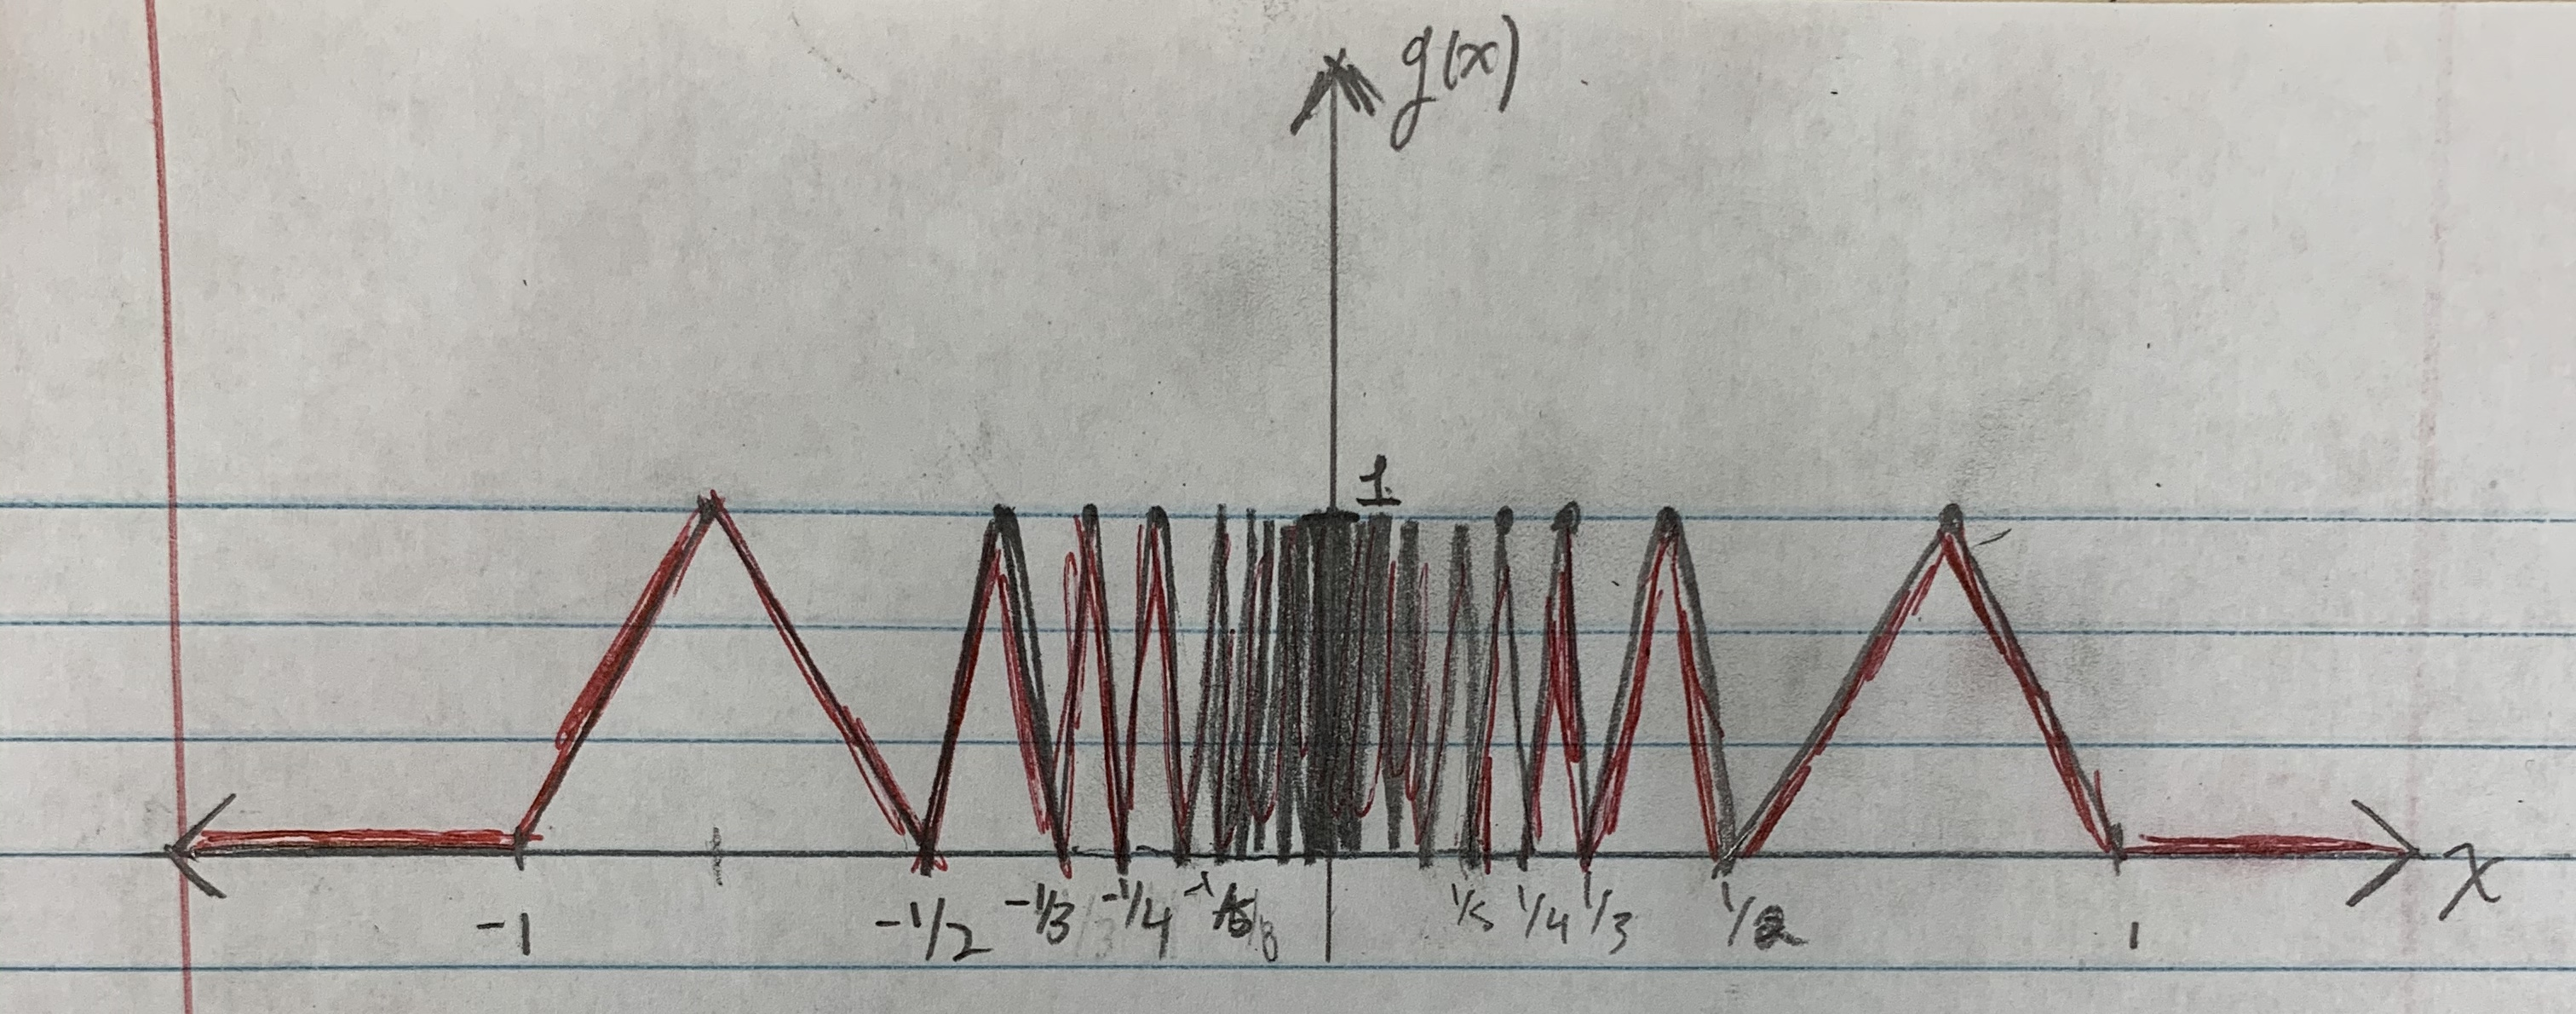
\includegraphics[width = \linewidth]{function_g.jpg}
\label{$g(x)$}
\end{figure}

Then $g$ is defined for all real numbers and $g(x) = f(x)$ for $x \in F$ (that is, $g\rvert_F = f$). So $g$ is an extension of $f$ to $\mathbb{R}$. Also, $g$ is continuous on $I_1$ and $I_2$ as $g$ is identically 0 on these open intervals. For each finite open interval $I_n = (a_n,b_n)$, $g$ is an increasing linear function on $(a_n, a_n + \frac{b_n-a_n}{2})$ and a decreasing linear function on $(a_n +\frac{b_n-a_n}{2}, b_n)$. Also, at the midpoint of each $(a_n,b_n)$, $a_n + \frac{b_n-a_n}{2}$,

$$1- \frac{2}{b_n-a_n}\left(a_n + \frac{b_n-a_n}{2} - \left(a_n + \frac{b_n-a_n}{2}\right)\right) = 1- \frac{2}{b_n-a_n}(0) = 1$$
$$\frac{2}{b_n-a_n}\left(a_n + \frac{b_n-a_n}{2} - a_n\right) = \frac{2}{b_n-a_n}\frac{b_n-a_n}{2}  = 1 \;.$$

So indeed the two lines used to define $g$ within any $I_n = (a_n,b_n)$ agree at a maximum of 1 at the midpoint of the interval. Therefore $g$ is continuous on each $I_n$. Also, at each endpoint $a_n$ and each endpoint $b_n$, we have
$$\text{lim}_{x \rightarrow a_n^+} g(x) = \text{lim}_{x\rightarrow a_n^+} \frac{2}{b_n - a_n}(x-a_n) = 0$$
$$ \text{lim}_{x\rightarrow b_n^-} g(x) = \text{lim}_{x\rightarrow b_n^-} 1 - \frac{2}{b_n - a_n}\left(x- (a_n + \frac{b_n-a_n}{2})\right) = 0 \;.$$

Since each $a_n,b_n \in F$ and $g(a_n) = g(b_n) = 0$, this shows that $g$ is continuous at each endpoint (recall also that $g \equiv 0$ on $(-\infty,-1)$ and $(1,\infty)$). Therefore, $g$ is continuous on $\overline{I_n}$ for each interval $I_n$ (this would only be an issue if we need to define $g$ on $\overline{R}$ for the case of $\overline{I_1}$, $\overline{I_2}$ but  this cannot be necessary since we are asked to find $g: \mathbb{R} \rightarrow \mathbb{R}$). As we proved in Homework 4, "$g$ is continuous on $\overline{I_n} \implies g\rvert_{\overline{I_n}}$ is continuous". \\

However, $g$ is not continuous at 0. Since $0 \in F$, $g(0) = f(0) = 0$. Consider $\epsilon = 1>0$ and let $\delta >0$ be arbitrary. Then there is a $k \in \mathbb{N}$ such that $k$ is even and  $k > 2/\delta + 2 \implies 0< 1/(k/2)< 1/(k/2 - 1) < \delta$. Thus we have an interval $I_k = \left(\frac{1}{k/2}, \frac{1}{k/2 - 1}\right) \subset (0,\delta)$ (we have $I_k = I_n= (a_n,b_n)$ for some $n$ but now it is more convenient to revert to the original notation). But then for the midpoint of this interval, $\alpha_k = 2/k + \frac{1}{2}\left(\frac{1}{k/2 - 1} - \frac{1}{k/2}\right)$, $g(\alpha_k)= 1$ using our definition of $g$. Therefore, there is an $\epsilon > 0$ (specifically $\epsilon = 1$) such that for every $\delta > 0$, we can find an $x$ ($\alpha_k$) such that $|x - 0| < \delta$ but $|g(x) - g(0)| = |1-0| = 1 \geq \epsilon$. Therefore $g$ is not continuous at $0$.

{\bf Proposition 17} Let $f$ be a real valued function defined and continuous on a closed and bounded set $F$. Then $f$ is bounded on $F$ and assumes its maximum and minimum on $F$; that is, there are points $x_1$ and $x_2$ in $F$ such that $f(x_1) \leq f(x) \leq f(x_2)$ for all $x \in F$.\\

Proof: Since $f$ is continuous on $F$, for each $x \in F$ there is an open interval $I_x$ such that $||f(y)| - |f(x)|| \leq |f(y) - f(x)| < \epsilon =1$ for all $y \in F\cap I_x$. Then $|f(y)| < |f(x)| + 1$ for all $y \in F\cap I_x$. The set $\{I_x : x \in F\}$ is an open cover of the closed and bounded set $F$. By Heine-Borel, there is a finite subcollection $\{I_{x_1},...,I_{x_n}\}$ such that $F \subset \cup_{i=1}^n I_{x_i}$. Let $M = 1+\text{max}\{|f(x_1)|,...,|f(x_n)|\}$. Then for any $y \in F$, we have $y \in I_{x_i}$ for at least one of the intervals. Then $|f(y)| < 1+|f(x_i)| \leq 1+\text{max}\{|f(x_1)|,...,|f(x_n)|\} = M$. This shows that $|f(y)| < M$ for all $y \in F$ and so $f$ is bounded on $F$ is bounded. \\

Assume $F \neq \emptyset$ so that $f(F) \neq \emptyset$. Then $f(F)$ is a nonempty bounded set. Let $\text{sup}_{x \in F} f(x) = m < \infty$. Suppose $f(x) < m$ for each $x \in F$. Then $0< (m-f(x))/2$ so by the continuity of $f$ there is an interval $I_x$ such that $f(y) - f(x) \leq |f(y)-f(x)| < m/2 - f(x)/2$ for all $y \in I_x \cap F$. From this $f(y) < (f(x) + m)/2$ for all $y \in I_x \cap F$. With these such intervals $F \subset \cup_{x \in F} I_x$ and again by Heine-Borel $F \subset \cup_{i=1}^n I_{x_i}$ for some finite subcollection. Set $a = \text{max}\{f(x_1),...,f(x_n)\}$. Then for each $y \in F$, since $y \in I_{x_i}$ for some interval from the finite subcover, $f(y) < (f(x_i) + m)/2 \leq (a+m)/2$. Thus $(a+m)/2$ is an upper bound of $f$ on $F$. But since $f(x) < m$ for all $x \in F$, $a = \text{max}\{f(x_1),...,f(x_n)\} < m$ and $(a+m)/2 < (m+m)/2 = m$. That is, $(a+m)/2$ is an upper bound of $f(F)$ that is less than the least upper bound of $f(F)$. This contradiction arose from supposing that $f(x) < m$ for each $x \in F$. So there is an $x_1 \in F$ such that $f(x_1) \geq m$ and since $m$ is an upper bound of $f(F)$, $f(x_1) = m \implies f$ attains its maximum value. A similar argument shows that there is an $x_2 \in F$ such that $f(x_2) = \text{inf}_{x \in F} f(x)$.  \\

{\bf Proposition 18} Let $f$ be a real valued function defined on $\mathbb{R}$. Then $f$ is continuous if and only if for each open set $\mathcal{O}$ of real numbers $f^{-1}[O]$ is an open set. \\

Proof: Suppose that for each open set $\mathcal{O}$ of real numbers $f^{-1}[O]$ is an open set. Let $x \in \mathbb{R}$ and $\epsilon > 0$. Since $(f(x) - \epsilon, f(x) + \epsilon)$ is an open set, $f^{-1}\left[(f(x) - \epsilon, f(x) + \epsilon)\right]$ is open. Then since $x \in f^{-1}\left[(f(x) - \epsilon, f(x) + \epsilon)\right]$ and this set is open there is a $\delta>0$ such that $(x - \delta, x+\delta) \subset f^{-1}\left[(f(x) - \epsilon, f(x) + \epsilon)\right]$. This means that for any $y \in \mathbb{R}$ with $|x-y| < \delta$, $y \in (x-\delta, x+\delta)$. So $y \in f^{-1}\left[(f(x) - \epsilon, f(x) + \epsilon)\right]$ and $f(y)\in (f(x) - \epsilon, f(x) + \epsilon) \implies |f(x) - f(y)| < \epsilon$. This shows that $f$ is continuous at $x$ and since $x \in \mathbb{R}$ was arbitrary conclude that $f$ is continuous on all of $\mathbb{R}$.\\

Suppose that $f: \mathbb{R} \rightarrow \mathbb{R}$ is continuous and let $O$ be an open set. We want to show that $f^{-1}[O]$ is open. Let $x \in f^{-1}[O]$ be arbitrary so that $f(x) \in O$. Since $O$ is open, there is an $\epsilon>0$ such that $(f(x) - \epsilon, f(x) + \epsilon) \subset O$. Since $f$ is continuous, there is a $\delta > 0$ such that if $|x-y|<\delta$ then $|f(x) - f(y)| < \epsilon$. Equivalently, if $y \in (x-\delta, x+\delta)$ then $f(y) \in (f(x) - \epsilon, f(x) + \epsilon)$. In general, if $A \subset B$, then $f^{-1}(A) \subset f^{-1}(B)$ ($x \in f^{-1}(A) \implies f(x) \in A$ $\implies f(x) \in B$ $\implies x \in f^{-1}(B)$) so we have $f^{-1}\left[(f(x) - \epsilon, f(x) + \epsilon)\right] \subset f^{-1}[O]$. Then if $y \in (x-\delta, x+\delta)$ we have $f(y) \in (f(x) - \epsilon, f(x) + \epsilon)$ and $y \in f^{-1}[O]$. That is, there is a $\delta>0$ such that $(x-\delta,x+\delta) \subset f^{-1}[O]$. Since $x \in f^{-1}[O]$ was arbitrary, conclude that $f^{-1}[O]$ is open. \\

{\bf Problem 42}
Let $(f_n)$ be a sequence of functions defined on a set $E$. Prove that if $(f_n)$ converges uniformly to $f$ on $E$, then $f$ is continuous on $E$. \\

Let $\epsilon>0$. Since $(f_n)$ converges to $f$ uniformly, there is an $N \in \mathbb{N}$ such that $|f_n(z) - f(z)| < \epsilon / 3$ for all $z \in E$ and $n\geq N$. In particular, $$|f_N(z) - f(z)| < \epsilon \text{ for all } z \in E \quad (1) \;.$$ Since $f_N$ is continuous, there is a $\delta > 0$ such that if $y \in E$ with $|x-y| < \delta$,
$$|f_N(x)-f_N(y)| < \epsilon / 3 \quad (2) \;.$$
Let $x \in E$. Then for any $y \in E$ with $|x-y|<\delta$,
\begin{align*}
|f(x) - f(y)| &= |f(x) -f_N(x) + f_N(x) -f_N(y) + f_N(y) - f(y)| \\
&\leq |f(x) -f_N(x)| + |f_N(x) -f_N(y)| + |f_N(y) - f(y)| \\
&< \underbrace{\frac{\epsilon}{3}}_{\text{By (1)}} + \underbrace{\frac{\epsilon}{3}}_{\text{By (2)}} +\underbrace{\frac{\epsilon}{3}}_{\text{By (1)}}\\
&= \epsilon \;.
\end{align*}

Since $x \in E$ was arbitrary $f$ is continuous on $E$. \\

{\bf Proposition 19 (Intermediate Value Theorem)} Let $f$ be a continuous real valued function on $[a,b]$ and suppose that $f(a) \leq \gamma \leq f(b)$ [or $f(b) \leq \gamma \leq f(b)$]; then there is a a point $c \in [a,b]$ such that $f(c) = \gamma$. \\
 
{\bf Problem 45} Prove Proposition 19. \\

Proof: Let $C = \{x \in [a,b] : f(x) < \gamma\}$. Since $a \in [a,b]$ and $f(a) < \gamma$, $C \neq \emptyset$ and since $C \subset [a,b]$, $C$ is bounded. Let $c = \text{sup } C$. If $f(c) > \gamma$, then since $f$ is continuous and $f(c) - \gamma > 0$, there is a $\delta > 0$ such that $f(y) > \gamma$ for all $y \in (c-\delta, c+\delta)$. But then we cannot have any point $x \in C$ with $x \in ( c- \delta, c+\delta)$ since otherwise $f(x) > \gamma$. But this contradicts the assumption that $c$ is the supremum of $C = \{x \in [a,b] : f(x) < \gamma\}$. So it must be the case that $f(c) \leq \gamma$. If $f(c) < \gamma$, then since $f$ is continuous and $0<\gamma - f(c)$ there is a $\delta > 0$ such that $f(y) < \gamma$ for all$y \in (c-\delta, c+\delta)$. But then there is an $x \in (c,c+\delta)$ such that $f(x) < \gamma$, which contradictions the assumption that $c$ is an upper bound of the set $C = \{x \in [a,b] : f(x) < \gamma\}$. So it cannot be the case that $f(c) < \gamma$ either. Therefore, conclude that $f(c) = \gamma$. Since $c$ is a cluster point of $C$ and $x\in [a,b]$ for all $x \in C$, the fact that $[a,b]$ is closed implies $c \in [a,b]$ as well. \\

Probably Incorrect Proof: If $\gamma = f(a)$ or $\gamma = f(b)$ then since $a \in [a,b]$ and $b \in [a,b]$ the conclusion holds. So suppose $f(a) < \gamma < f(b)$. Then $(f(a),f(b))$ is an open set and $\gamma \in (f(a),f(b))$. There is an $\epsilon > 0$ such that $(\gamma - \epsilon, \gamma + \epsilon) \subset (f(a),f(b))$. Then for any $n \in \mathbb{N}$ with $1/n<\epsilon$ it follows that $(\gamma-1/n, \gamma + 1/n) \subset (f(a),f(b))$. Since $f$ is continuous, $f^{-1}((\gamma-1/n, \gamma + 1/n)) \subset (a,b)$ (what if this is empty?) is open by Proposition 18 (while Proposition 18 is stated with a function defined on the real line, we saw in Problem 40 that it is possible to find a continuous extension of $f$ to the real line that matches $f$ on the compact set $[a,b]$ so we will continue to just use $f$ in this proof instead of the extension $g$). Then for each $n$ with $n<1/\epsilon$ take $x_n \in f^{-1}((\gamma-1/n, \gamma + 1/n))$ to construct the sequence $(x_n)$. Since $x_n \in [a,b]$ for all $n$ and $[a,b]$ is a closed and bounded set, there is a subsequence $(x_{n_k})$ of $(x_n)$ such that lim $x_{n_k} = c \in [a,b]$. Then lim $f(x_{n_k}) = f(c) = \gamma$ since $f$ is continuous. \\

{\bf Definition} A real valued function $f$ defined on a set $E$ is said to be uniformly continuous on $E$ if given $\epsilon > 0$ there is a $\delta > 0$ such that for all $x$ and $y$ in $E$ with $|x-y| < \delta$ we have $|f(x) - f(y)| < \epsilon$. \\

{\bf Proposition 20} If a real valued function $f$ is defined and continuous on a closed and bounded set $F$ of real numbers, then $f$ is uniformly continuous on $F$. \\

Proof: Given $\epsilon > 0$ we have for any $x \in F$ a $\delta_x$ such that for $y \in (x-\delta_x/2,x+\delta_x/2) =: I_x$, $f(y) \in (f(x) - \epsilon/2, f(x) + \epsilon/2)$. This gives the open cover $\cup_{x \in F} I_x \supset F$. Since $F$ is closed and bounded there is a finite subcover $\cup_{i=1}^n I_{x_i} \supset F$. Let $\delta = \text{min}\{\delta_{x_1}, ..., \delta_{x_2}\} / 2$ and let $y,z \in F$ with $|y-z| < \delta$. Then $y \in I_{x_i}$ for an open interval in the finite subcover and $z \in I_{x_j}$ for an open interval in the finite subcover, although it may be that $i \neq j$. Since $y \in I_{x_i}$, $|f(y) - f(x_i)| < \epsilon/2$. Since $|z-x_i| = |z - y + y - x_i| \leq |z-y| +|y-x_i| < \delta + \delta_{x_i}/2< \delta_{x_i}/2 + \delta_{x_i}/2 = \delta_{x_i}$, it is also the case that $|f(z) - f(x_i)| < \epsilon/2$. Therefore $|f(z) - f(y)| \leq |f(z) - f(x_i)| + |f(x_i) - f(y)| < \epsilon/2 + \epsilon/2 = \epsilon$. This shows that for $\epsilon > 0$ there is a $\delta>0$ such that whenever $y,z \in F$ and $|y-z| < \delta$ it follows that $|f(y) - f(z)| < \epsilon$. Therefore $f$ is uniformly continuous on $F$. \\

\end{document}